 
\documentclass[10pt,journal,compsoc]{IEEEtran}


% *** CITATION PACKAGES ***
%
\usepackage[pdftex]{graphicx}
\usepackage{framed}
\usepackage{colortbl}
\usepackage{multirow}
\usepackage{subfigure}
\usepackage{xspace}
\usepackage{amssymb}
\usepackage{tabularx}
\usepackage{caption}
\usepackage{subcaption}
\usepackage[english]{babel}
\usepackage{ragged2e}
\usepackage{blindtext}
\usepackage{adjustbox}
\ifCLASSOPTIONcompsoc
  % The IEEE Computer Society needs nocompress option
  % requires cite.sty v4.0 or later (November 2003)
  \usepackage[nocompress]{cite}
\else
  % normal IEEE
  \usepackage{cite}
\fi
% *** GRAPHICS RELATED PACKAGES ***
%
\ifCLASSINFOpdf
  % \usepackage[pdftex]{graphicx}
  % declare the path(s) where your graphic files are
  % \graphicspath{{../pdf/}{../jpeg/}}
  % and their extensions so you won't have to specify these with
  % every instance of \includegraphics
  % \DeclareGraphicsExtensions{.pdf,.jpeg,.png}
\else
  % or other class option (dvipsone, dvipdf, if not using dvips). graphicx
  % will default to the driver specified in the system graphics.cfg if no
  % driver is specified.
  % \usepackage[dvips]{graphicx}
  % declare the path(s) where your graphic files are
  % \graphicspath{{../eps/}}
  % and their extensions so you won't have to specify these with
  % every instance of \includegraphics
  % \DeclareGraphicsExtensions{.eps}
\fi

\newcommand\MYhyperrefoptions{bookmarks=true,bookmarksnumbered=true,
pdfpagemode={UseOutlines},plainpages=false,pdfpagelabels=true,
colorlinks=true,linkcolor={black},citecolor={black},urlcolor={black},
pdftitle={Bare Demo of IEEEtran.cls for Computer Society Journals},%<!CHANGE!
pdfsubject={Typesetting},%<!CHANGE!
pdfauthor={Michael D. Shell},%<!CHANGE!
pdfkeywords={Computer Society, IEEEtran, journal, LaTeX, paper,
             template}}%<^!CHANGE!

\newcommand\jp[1]{\textcolor{blue}{Justyna: #1}}
\newcommand\ls[1]{\textcolor{red}{Leandro: #1}}
\newcommand\pl[1]{\textcolor{red}{Paulo: #1}}

\newcommand\esa[1]{\textcolor{green}{Eduardo: #1}}
\newcommand{\todo}[1] {{\color{red} \textbf{[TODO: #1]}}}
\newcommand{\autoscalpel}{\textsc{prodScalpel}\xspace}
\newcommand{\FOUNDRY}{\textsc{Foundry}\xspace}

% correct bad hyphenation here
\hyphenation{op-tical net-works semi-conduc-tor}


\begin{document}

\title{Automated Reengineering of Systems into SPL\\ via Software Transplantation}
%\ls{Suggestion of new title: "Automated migration of software systems to SPL via Software Transplantation"}}

\author{Author~1,~\IEEEmembership{Member,~IEEE,}
        Author~2,~\IEEEmembership{Fellow,~OSA,}
        and~Author~3,~\IEEEmembership{Life~Fellow,~IEEE}% <-this % stops a space
\IEEEcompsocitemizethanks{\IEEEcompsocthanksitem M. Shell was with the Department
of Electrical and Computer Engineering, Georgia Institute of Technology, Atlanta,
GA, 30332.\protect\\
% note need leading \protect in front of \\ to get a newline within \thanks as
% \\ is fragile and will error, could use \hfil\break instead.
E-mail: see http://www.michaelshell.org/contact.html
\IEEEcompsocthanksitem J. Doe and J. Doe are with Anonymous University.}% <-this % stops a space
\thanks{Manuscript received April 19, 2005; revised August 26, 2015.}}


% The paper headers
\markboth{Journal of \LaTeX\ Class Files,~Vol.~14, No.~8, August~2015}%
{Shell \MakeLowercase{\textit{et al.}}: Bare Advanced Demo of IEEEtran.cls for IEEE Computer Society Journals}

\IEEEtitleabstractindextext{%
\begin{abstract}\justifying \pl{eu acho que ainda no abstract voce deveria deixa explicito que a contribuicao é tanto uma abordagem quanto uma ferramenta. E que novas ferramentas, considerendo outras linguagens podem ser desenvolvidas para dar suporte a abordagem. }
Software Product Line (SPL) is a software reuse approach that improves time-to-market and software quality, achieving substantial cost reductions. These benefits do not come for free. It often takes years to rearchitect and reengineer a code base to support SPL and, once adopted, it must be maintained. Current practice relies on a collection of tools, tailored for different reegineering phases, whose output developers must coordinate \pl{coordenada e integrada. A saida de uma deve servir como entrada para outra ferramenta}. To speed conversion \pl{and creation} to and maintenance of SPL, we present \FOUNDRY, the first software transplantation approach that transplants and merges features from different systems without creating or manually adapting the assets specifically for an SPL, as the assets are collected from diverse existing systems and automatically adapted. We realised \FOUNDRY~in \autoscalpel, a software transplantation tool for SPL that facilitates feature identification and can efficiently transplant a multi-organ, i.e., a sequence of features. We used \autoscalpel to create two product lines that integrate features from three real-world systems each. We also conducted an experiment comparing it with manual effort. The results show that \autoscalpel is able to migrate features between different codebases within 4.8 times faster \pl{foi so rapido? A qualidade nao melhorou?} than the mean of participants, a group of 20 SPL experts. 

\end{abstract}

% Note that keywords are not normally used for peerreview papers.
\begin{IEEEkeywords}
Computer Society, IEEE, IEEEtran, journal, \LaTeX, paper, template.
\end{IEEEkeywords}}


\maketitle

\IEEEdisplaynontitleabstractindextext

\IEEEpeerreviewmaketitle

\section{Introduction}
\label{sec:introduction}

Software Product Line (SPL) engineering has emerged as a systematic methodology for producing related software products from shared development assets~\cite{Pohl2005, Linden2007, Fischer2015}.
SPL organises a codebase into a set of shared features, a dependency relation over those features, and defines a variability mechanism that creates products from subsets of the features subject to the dependency relation.
By centralising features into a shared set, SPL prevents feature drift, allowing all products to benefit from a feature's improvement, if they use it.
For companies producing related products, adopting SPL improves productivity and quality, speeds time to market, and reduces cost, because it permits systematic reuse of development artifacts, such as code and design~\cite{Linden2007,Bastos2015}.

Despite its benefits, adopting SPL requires considerable upfront investment before those benefits can be realised. 
The cost to migrate existing products to SPL is even higher than adopting SPL from scratch, yet most SPL adoption is extractive --- it re-engineers an existing codebase~\cite{Krueger2001, Berger2013}. \pl{essa referencia fala que o custo de fazer uma spl com base em algo existente é maior que fazer do zero?}
Two factors drive this preference: greenfield adoption of SPL is uncommon because related products often emerge from a small set of initial products, while starting from scratch discards considerable  knowledge and investment in existing codebases~\cite{Breivold2008,Northrop2012}.

To re-engineer existing products, companies must solve four problems:  They must analyse the products to 1) identify and 2) extract the features these products share and 3) learn their inter-dependencies; finally, they must 4) define a variability mechanism for combining these features, subject to their inter-dependency constraints~\cite{Assuncao2017}.
Each of these tasks, alone, is challenging; together, they are extremely complex.
Thus, it is not surprising that re-engineering to adopt SPL remains largely manual~\cite{Biggerstaff1993, Kastner2011, Lopez2011} and costly~\cite{Bockle2004}.
Indeed, because of its cost, software companies delay, or even refrain from, adopting SPL~\cite{Fischer2015}.
Assunção et al.'s excellent survey~\cite{Assuncao2017} identifies the key challenges of SPL re-engineering.  
Three technical challenges, in particular, concern us here:  automation and tool support,  improved feature management, and the lack of sophisticated refactoring.

In 2013, Harman et al.~\cite{Harman2013} introduced software transplantation (ST) as a new research direction and laid out its implications for SPL re-engineering. Harman et al. defined software transplantation as ``\emph{the adaptation of one system's behaviour or structure to incorporate a subset of the behaviour or structure of another}''~\cite{Harman2013}.
Software transplantation defines a new means to automatically move all the code fragments that make up a feature between codebases, even unrelated ones. 

Inspired by this vision, we introduce \FOUNDRY, the first software transplantation methodology for SPL re-engineering.
\FOUNDRY addresses each of the three technical challenges Assunção et al. identified, for each of the four SPL tasks. \FOUNDRY does not eliminate the manual labour of feature identification, but reduces it to the task of annotating the entry points (i.e. the interface) of a feature, or ``organ'' using transplantation nomenclature. \FOUNDRY does, however, amortise this manual step across multiple transplantations. Given an entry point, \FOUNDRY uses conservative slicing to automatically extract a feature into an ``overorgan'', completely automating the extraction task. \FOUNDRY's conservative slicing also implicitly learns a feature's dependencies, by including them in its overorgan.
Finally, \FOUNDRY uses software transplantation's implantation stage as its variability mechanism --- it produces a new product by transplanting the features it needs into a host product base without any kind of annotation. 

\FOUNDRY's variability mechanism, implantation, combats the bloat and redundancy of its conservative solution to SPL's dependency task:  it uses clone-aware genetic improvement~\cite{Petke18:genetic} to reduce and adapt the overorgan to an organ appropriate to the host product's context.
This implantation process uses clone detection to discard redundant, overlapping dependencies that may exist across two overorgans. \FOUNDRY's variability mechanism also supports surrounding implanted organs with feature flags or preprocessor directives, which permit enabling and disabling features, to facilitate its integration into an existing SPL codebase that uses them.

We realise \FOUNDRY in \autoscalpel, a tool that transplants multiple organs (i.e., a set of interesting features) from possibly distinct donor systems into an emergent product line. It is the first tool to apply software transplantation to SPL re-engineering.
%%%\ls{ Reviewer#3: The introduction is way to long and should be shortened. In particular, I find the different scenarios described to motivate the benefits of ProdScalpel (l.140-160) really hard to follow, mainly because it is too short and leaves many aspects open. Better to remove them here and keep the introduction focused and simple.}

\autoscalpel supports various SPL re-engineering scenarios. First and simplest, \autoscalpel can automate clone-and-own~\cite{Dubinsky2013, Fischer2015}, especially the task of synchronising changes to a feature shared across two products created by clone-and-own. For example, consider the case where the copy of a shared feature in one of the two products is patched to fix a bug. \autoscalpel permits transplanting the fixed version over the top of the unpatched copy of the feature in the other product. Second, companies can use \autoscalpel just for the initial conversion of an existing codebase into SPL. In this mode, \autoscalpel first extracts overorgans from the donor systems, then produces a product base, created from an existing system by removing all unwanted features to the product line. Then, implants the overorgans into this product base, identifying and removing cross-overorgan redundancies. The resulting organs becomes the SPL's shared set of features. \autoscalpel can itself be used as a variability mechanism to construct new products by implanting features into a product base. Even with this one-off application of \autoscalpel, the company also can then use a conventional variability mechanism. For existing SPL codebase, such as one it created. Finally, \autoscalpel permits a wholly new form of SPL, \emph{symbiotic SPL}:  in this mode, the donor can be oblivious to a parallel, ongoing SPL reorganisation of its codebase. To capture improvements in the donor, \autoscalpel periodically refreshes its set of features by re-transplanting them into its donor product base and thence into host products. For instance, one could use \autoscalpel to produce lightweight, specialised text editors from the \emph{Vim} project. \pl{Eu acho que vale a pena destacar os cenarios onde a ferramenta pode ser utlizada no contexto de SPL. O texto ta denso. Eu colocaria (i)(ii)(iii)}     

To evaluate \FOUNDRY~and \autoscalpel, we conducted two case studies and a controlled experiment. We first generate products by transplanting features from three real-would systems ---  Kilo\footnote{https://github.com/antirez/kilo}, VI\footnote{http://ex-vi.sourceforge.net/} and CFLOW\footnote{https://www.gnu.org/software/cflow/} --- into two product bases generated from VI and VIM\footnote{https://www.vim.org/}, used as hosts for the target transplantations. Next, we asked twenty SPL experts to conduct a experiment of feature migration to a product line. We gave them the same input as the one required by \autoscalpel. In all cases \autoscalpel outperformed our experiment's participants in the time taken to complete feature migration.

Our results provide evidence to support the claim that automated product line generation, using software transplantation, is a feasible and, indeed, promising approach for automated product development, containing functionality from existing, possibly unrelated, systems.

The main contributions of this paper are: 
\begin{enumerate}
    \item \FOUNDRY, a new SPL re-engineering methodology based on software transplantation and its realisation in \autoscalpel;
    \item A rigorous evaluation of \autoscalpel that demonstrates \FOUNDRY's promise; we use \autoscalpel to generate two product lines, and two new products, composed of features transplanted from three different real-world codebases.
    \item An experiment that shows that \autoscalpel migrates features 4.8 faster on average than SPL experts performing the same task, \emph{when the developers managed to complete the task}, both using testing to validate the migrated features; this result demonstrates \autoscalpel promise for improving SPL adoption. \pl{o resultado so mostra o aspecto da velocidade que foi maior? tem algo a adicionar sobre a qualidade do codigo? dead code?Alem disso a ferramenta pode ser usada tanto no cenario de criacao quanto de manutencao de codigo na SPL}
\end{enumerate}

 

\section{Motivating Example} \label{sec:motivating_example}


We chose the open-source GNOME project\footnote{https://wiki.gnome.org/Projects} as our motivating example. GNOME  project encompasses a large portfolio of individual programs, separately maintained. These programs share features, but GNOME cannot easily reuse features across its portfolio. It is a natural candidate for SPL, but has not adopted it, because of the prohibitive cost of this task.  \FOUNDRY is transformative because it can be used to reduce the cost of adopting SPL.

We now show how to GNOME team can apply \FOUNDRY to quickly generate one or more product lines, using \autoscalpel. Suppose project collaborators want to build a product line in the domain of text editors using \FOUNDRY to reuse features from existing systems. This product line would make GNOME project able to produce customized text editors with features that its current text editor, \emph{GEdit}\footnote{https://wiki.gnome.org/Apps/Gedit}, lacks. We assume that the GNOME team has determined that there is a market/demand for such a product and targets the following three features (1) $\texttt{side-panel}$, (2) $\texttt{split pane}$, and (3) $\texttt{presentation}$. They then identify two donors from which to transplant these features:  \emph{NEdit}\footnote{https://sourceforge.net/projects/nedit/}, a multi-purpose text editor, and \emph{Evince}\footnote{https://wiki.gnome.org/Apps/Evince}, a document viewer for multiple document formats. 
 
The process is executed in an iterative and incremental fashion by using \autoscalpel. In the first step (in a preoperative stage) the donors and the host are prepared for the transplantation process. For the donor's preparation, \autoscalpel is used by GNOME engineers to remove all portions of code surrounded by preprocessor directives. Although useful for donor programs, some conditional directives, if transplanted, will generate dead code — unnecessary code fragments~\cite{Tartler2011} that will never be included in any valid feature selection. For the host preparation, a \emph{product base} needs to be selected from existing systems. A  product base is used as a core of the product line, serving as a host for features to be transplanted. 

The GNOME development team then selects GEdit as a product base for the target product line. It is chosen for already had some commonalities (i.e. common features) among the products to be derived from the GNOME product line. However, GEdit has unwanted features for the product line portfolio that need to be removed. This task is usually costly, tedious and error-prone, if done manually. \autoscalpel provides an automated way for removing optional features from a product base when it is implemented with preprocessor statements like \#IFDEFS in C and C++. 

Once they have the product base from GEdit, the developers must then augment it with annotations to demarcate implantation points for each target feature, or “organ” using transplantation nomenclature. They also need to demarcate organ entry points for each one to be transplanted. Note that the features do not need to be explicitly defined, using preprocessor directives or any other mechanism. \autoscalpel only requires annotation of the entry point of the method implementing the desired feature. 

The pre-operative process produces a product base, adapted to receive all variant features transplanted from the donor programs. Then, the engineers can run \autoscalpel to transplant the three features targeted above. For each feature, \autoscalpel automatically extracts all of that feature's source code and its dependencies, or “over-organ” using transplantation nomenclature, using \emph{program slicing}~\cite{Binkley:2014:OLP:2635868.2635893} technique. The extracted over-organ is added to an \emph{Icebox} repository, a repository from which over-organs are kept to be reused by using the transplantation process.

For producing new product variants, \autoscalpel implements an observational slicing in Genetic Programming (GP)~\cite{Harman2009} that reduces the organ and adapt it to execute in the product base. \autoscalpel first transplants the \emph{side-panel} feature, extracted from GEdit itself. This transplantation demonstrates that \autoscalpel can transplant features into a product base that comes from the same codebase. It shows how developers can use \autoscalpel to produce a customized product from a single product base. Next, \autoscalpel transplants the \emph{split\_pane} feature from NEdit, which is an editor like GEdit, but not part of the GNOME portfolio. It shows how \autoscalpel manage to transplant features from distinct codebases, which is not possible without manual effort using the current state-of-art to SPL re-engineering. Finally, \autoscalpel transplants the \emph{presentation} feature from the Evince program, which is a GNOME project, but not a text editor. %Figure~\ref{fig:incremental_pd} illustrates this process. 

Using \FOUNDRY different products variants may be derived from a thus created product line upon request by using software transplantation. The transplantation technique applied by \FOUNDRY generates a representation of an SPL implementation without any annotated code. The annotation-based representation suffers from its negative effect on code understanding, maintainability and error proneness when many annotations appear in the code. Annotated code can become unreadable and hard to be maintained~\cite{Nicolas2021}. This is often referred to as the \emph{if/else hell} problem~\cite{Tartler2011, Aleixo2012, Medeiros2015}. %~\cite{Tartler2011}. 

We envision two ways of maintaining such created product line. 
Firstly, one can re-transplant the features if the original source codebase changes. This is thus already supported by \autoscalpel.
Secondly, one can maintain the extracted over-organs, and re-run the adaptation and implantation stages, as need be. \pl{tu acha q vale a pena colocar a palavra maintaining em negrito para destacar mais? como o texto ta grande e denso eu acho que vale a pena destacar de alguma forma. Italico}

\FOUNDRY can also be exploited as an alternative to directly generating variants of GEdit. For this, \autoscalpel can be used to create a single product by transplanting these target features in the original version of GEdit, without any variability mechanism.

\FOUNDRY can open the door to transplanting features from any program  into a product line, scaling up feature reuse. 
% throughout the  product portfolio. 
Open-source projects, like GNOME, are a promising source of code for the concept of software transplantation for SPL reengineering. Open-source code enables every developer the opportunity to share code, allowing them to migrate an already existing code from a pre-existing source into their own SPL project.


\section{Multi-organ Transplantation}\label{sec:background}

Automating software transplantation involves inserting portions of code from an organ into the target site in the host~\cite{Barr2015}. Barr et al. showed its effectiveness in transplanting code both between different versions of the same system~\cite{Petke2014} and between two different systems~\cite{Barr2015}. Nevertheless, to make the application of this technique in generating SPL feasible, we must consider the transplantation of multiple organs from possibly distinct donors into a single host codebase.

In practice, an organ implementing the functionality in a system often shares elements, such as variables, declarations, functions, etc., with one or more other organs. For instance, a structure that stores data manipulated by more than one function. Dealing with this kind of dependency is not necessary when only a single organ is migrated. This indicates a marked difference between the initial solution implemented by Barr et al. and our ST approach. This particular aspect presents a new challenge in the software transplantation field for SPL generation, handled by our approach.

\section{Foundry}
\label{sec:approach}

In this section, we present \FOUNDRY's workflow. Figure~\ref{fig:approach} overviews \FOUNDRY and how it is automated by \autoscalpel. Given an organs' entry point for the organ in the donor systems, its target implantation point in the product base, and a test suite that exercise the organ, it automatically: extracts an over-organ; constructs an organ-host compatibility layer; transforms the organ to be compatible with the context of its target sites in the product base; and implants it in the beneficiary's environment. All product derivation processes are performed in an iterative way where each organ is transplanted step-wise, and a new product is incrementally constructed as each organ is extracted and successfully transplanted. 

\begin{figure*}[t]
	\centering  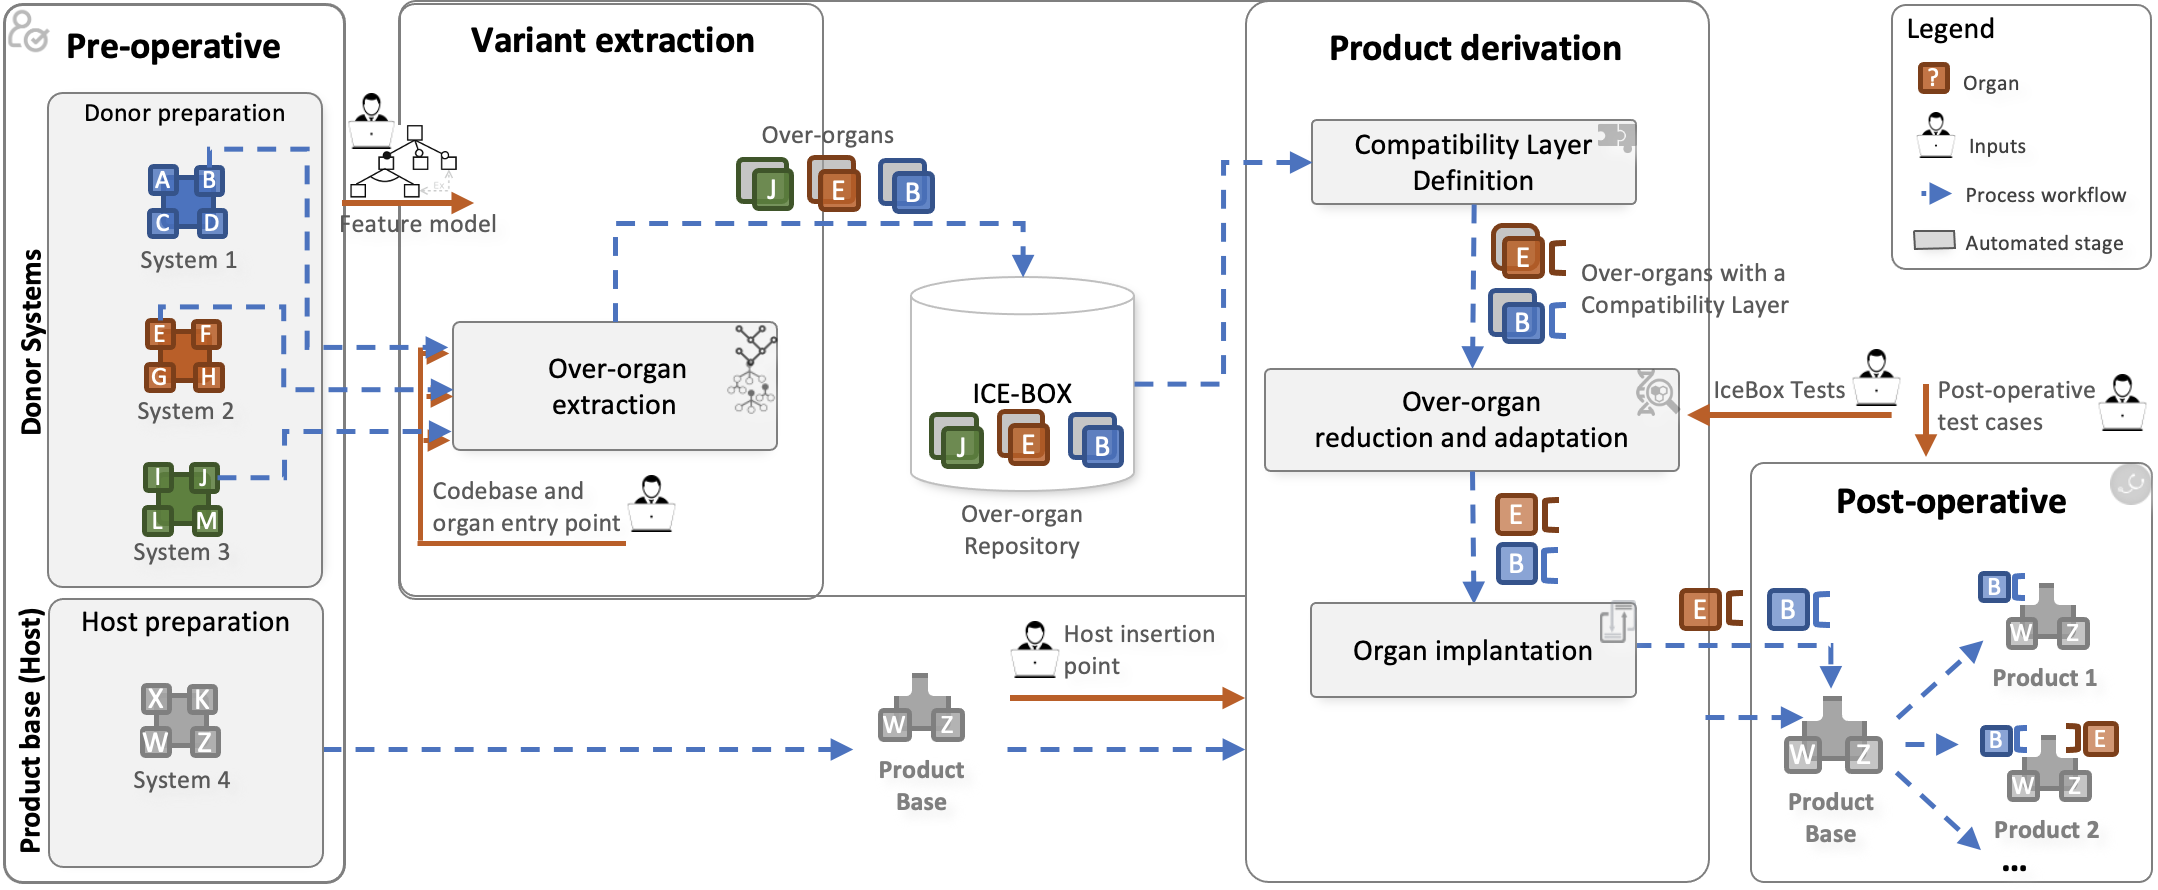
\includegraphics[width=18.5cm]{images/FOUNDRY3.png}
	\centering \caption{Overview of ST for generating product lines.}
	\label{fig:approach}
\end{figure*} 

Currently, \FOUNDRY is realized by \autoscalpel. The tool was implemented to generate product line representations from codebases written in C, however, the \FOUNDRY approach can be extend its scope to be used in the transplanting of features from codebases written in other languages. In this  section,  we provide details on the approach and how it is implemented by \autoscalpel

\subsection{Preoperative Stage} \pl{na figura tu colocou Pre-Operative}

As in medicine, our approach requires a \emph{preoperative} stage where donors and the host are prepared for the transplantation process and a \emph{postoperative} stage where the successful transplantation degree is evaluated. The preoperative stage defines a set of pre-transplantation tasks, responsible for the variability analysis process as well as the organ's test suite preparation. 

\subsubsection{Variability Analysis}

The preoperative stage starts with a variability analysis process in the donor candidates to discover features in existing products with the potential to compose the target product line. This task aims to create the variability model to express the valid combinations of features among the donor systems from which they will be extracted.  The variability model can be represented by using a feature model~\cite{Kang1990}.

Each feature representation in the feature model is annotated with 
its correspondent entry point (an organ entry point) in the donor codebase. An organ's entry point is a function in the donor systems that definitely belongs to the organ and defines correctly an execution environment expected for its initialization and provides the correct access to the organ's test suite. To determine the organ’s entry point, the user needs to provide the name of the function to \autoscalpel. 

\subsubsection{Donor Preparation}

Before starting the transplantation, the user selects a set of donor programs to provide features to the product line.It is spectated that one or more of those codebases can have annotations (e.g., code fragments guarded by \#ifdef C-preprocessor directives~\cite{Tartler2011})  commonly used to control code extensions related to features. Although useful for the donor program, such annotations, if transplanted, will generate dead code—fragments~\cite{Tartler2011} that will never be included in any valid feature selection. 

Using its \emph{Reconfigurator} and a textual list of preprocessor directives annotated with the prefix $\texttt{-D}$ provided by the user, \autoscalpel avoids these collateral effects by cleaning up unused directives and associated dead code from the donors. Thus, conditional directives belonging to the target organs are not transplanted to the host. This is done in a way that preserves as much of the source code structure belonging to the organ (indentation, spacing, number formats, etc.) as possible, to prevent future bugs. Figure~\ref{fig:reconfigurator} gives a example of a portion of code after \autoscalpel clean up unused directives.

\begin{figure}[t]
	\centering 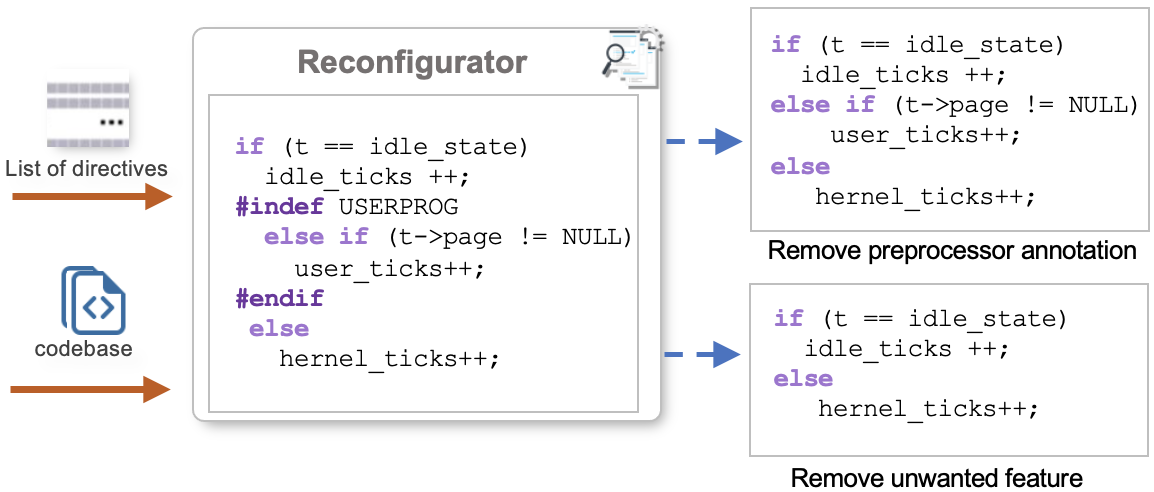
\includegraphics[width=9cm]{images/reconfigurator.png}
	\centering 
	\caption{The reconfigurator used to automated removal of preprocessor annotation from donor codebase and unwanted features from product base.}
	\label{fig:reconfigurator}
\end{figure} 

\subsubsection{Host preparation}

Still, during the pre-operative stage, the user has to select a product base from some existing system. If well-chosen, a product base can already provide a set of solutions so close to the target products that it can be used as a baseline for the assembly of the products to be generated. For example, a text edition program could provide a baseline for new programs for text translation,  presentation or rendering, since they could have a considerable number of common features among them.

The idea behind of product base is to take simultaneous advantage of commonality to reduce effort by transplanting only specific features required by each product variant. That is, while the product base provides commonalities (i.e. common features) to the target product line, the variabilities (i.e. variant features) are provided by the transplantation process, as illustrated by Figure~\ref{fig:product_for_transplantation}.

Case necessary the product base can be reduced to its basic form, keeping only mandatory or features relevant to the target product line. The reduction process consists of removal of all code that implements all features which will not be required to compose the product line. \autoscalpel's reconfigurator has been implemented to give support for the automatic feature removal from a codebase implemented using a mechanism like preprocessor directives. Such a mechanism allows the automatic identification and isolation of all fragments of code associated with a particular feature delimited such directives. 

\begin{figure}[t]
	\centering 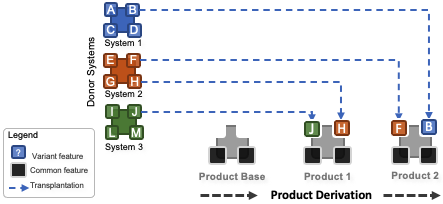
\includegraphics[width=\columnwidth]{images/product_for_transplantation.png}
	\centering 
	\caption{A product base used to generate different products.}
	\label{fig:product_for_transplantation}
\end{figure} 

To automate the feature removal process, \autoscalpel initially requires the user to provide as input a textual list of directives annotated with the prefix $\texttt{-U}$, corresponding to each feature to be removed. \autoscalpel then maps and searches selectively for pieces of code that implement features limited by such directives. Then, \autoscalpel removes all features source code from the product base while it keeps the source code structure belonging to the product base unchanged and ready to receive the transplanted organs.

In a removal scenario where the product base is implemented without a variability mechanism, additional attention is necessary to find and remove all portions of code that implement a target feature without compromising the codebase.

%%Note that a product base, once reduced, can be used multiple times as a base for new products. Although its preparation may require considerable effort for localising and removing all unnecessary code, it can be compensated with the benefits achieved through using the product base as a baseline to build other products belonging to the same or similar domain.

\subsection{Organ Test Suite Preparation}

For the transplantation process, the user also must supply test suites, called \emph{ice-box tests}~\cite{Barr2015}. They are used to guide GP in the search for extracted code modifications required to make the organ fully executable when implanted in the product base (see section~\ref{sec:organ_reduction}). The ice-box tests are implemented as \emph{in-situ}, a form of unit testing that starts from a valid program state rather than an arbitrary state~\cite{Barr2015}. Easily implementable, using the \emph{Check} unit testing framework for C~\cite{Check2019}, for instance, \emph{in-situ} unit testing allows us to leverage a single path to rigorously test whether the new functionality executes correctly in the host environment. 

Although ice-box tests can be quick to develop, it can be implemented using some existing test generation tools for C, or even adapted from donor’s unit tests to the host’s execution environment. 

\subsection{Over-organ Extraction}
Once the preoperative is stage done, and all inputs are prepared, we can start the automated organ extraction and transplantation process, using \autoscalpel. The code extracting process is a critical issue since it also involves identifying all semantically required code elements for the organ to be kept functional, even outside its original codebase. That way, the extraction of a target organ captures a considerable amount of code at different levels of granularity, from moving required files and libraries to entire functions and individual statements, both potentially not confined to a single file or library~\cite{Petrenko2009}.

We implemented a hybrid~\cite{Assuncao2017} process of extraction that uses a new kind of  GP, augmented by a form of dynamic observational slicing~\cite{Barr2015}, which we extended to compute slices from multiple files. The process of slicing discards those parts of the donor program that can be determined to have no effect upon the organ. Hence, it allows us to obtain an executable subset of program statements that preserves the original behaviour of the organ from its entry point in the donor program.

Figure~\ref{fig:over-organ_extraction} illustrates the slicing process. Technically, \autoscalpel builds call and caller graphs for each function implemented in the donor system. Then, it selects the call graphs corresponding to the organ's entry point. The organ's entry point is used as a starting point for automated organ slicing.

Using the observation-based slicing approach~\cite{Binkley:2014:OLP:2635868.2635893}, \autoscalpel reaches all functions from the organ's entry point. To find the over-organ, it slices forwards by isolating the donor's call graph edges that are particularly relevant to the organ under consideration. To compute a slice, it context-insensitively traverses the donor's call graph and transitively includes all the functions called by any function whose definition it reaches. The result is a set of slices that, when combined, produce an \emph{over-organ} that conservatively over-approximates the target organ~\cite{Barr2015}.

\begin{figure}[t]
	\centering 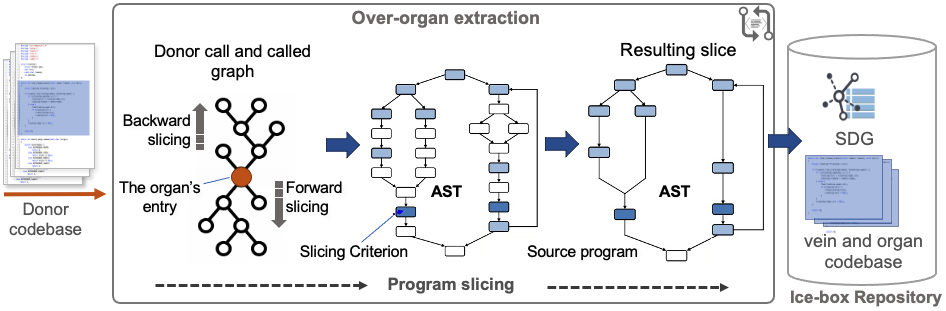
\includegraphics[width=\columnwidth]{images/over-organ_extraction2.png}
	\centering 
	\caption{Over-organ extraction process}
	\label{fig:over-organ_extraction}
\end{figure} 

The target organ implements the functionality to be transplanted; however, to be correctly initialized and executed, it requires an execution environment, called the vein~\cite{Barr2015} that correctly constructs the organ's parameters at its entry point. In the donor context, the execution environment is provided by one or more execution paths, that start at the donor's entry point (generally the function $\texttt{main}$) and ends at the organ's entry point. To compute a vein for an organ, \autoscalpel~slices backwards from the given organ's entry point traversing the call graph in reverse until it reaches the donor's entry point. Once it reaches the donor's entry point, \autoscalpel~prunes the slice to retain only the shortest path, under the assumption that all paths to the organ are equivalent. 

Once an over-organ is extracted, \autoscalpel~builds the donor's System Dependence Graphs (SDG)~\cite{Horwitz1988} which is used by GP to constrain its search space and to reject syntactically invalid offspring. Every function belonging to the call graph is represented as a dependency graph. Based on~\cite{Horwitz1988}, SDG includes data-dependence edges that represent transitive dependencies between function calls, in addition to the conventional direct-dependence edges. 

At the end of the extraction process, both organ and vein are kept in an IceBox repository to be, posteriorly, transplanted to the product base, deriving new product variants. 

\subsection{Compatibility Layer Definition}

Now we can start the derivation process when the target organ is then selected from Icebox to be pruned, adapted and implanted into the product base environment.

Harman et al.~\cite{Harman2013} proposed the construction of an interface between the transplant and the host into which candidate transplants can be initialized and evaluated. Following their proposal, we have introduced an \emph{organ-host converter}, a layer that works as a kind of organ-host interface responsible for providing access to the organ from the host.

The process of defining the interface is automated by using GP algorithm. It requires the correct mapping the parameters of the host-side implantation-point to the argument required by the organ's interface signature.Thus, the challenge for the GP algorithm is to efficiently find a binding between the host’s variable in scope at the implantation point inside the host to the organ’s interface parameters that correctly initialize an execution environment expected by the organ and provide the correct access by the organ’s tests. Some of these variables will need to be created and initialized during GP-refinement; others will use existing host variables. 

In practice, \autoscalpel inserts a call to the converter at the implantation point in the host. In the interface, \autoscalpel~ abstracts variable names so that GP can select a type-compatible binding. It selects different combinations of all valid statements and variables mapped from the organ's vein to initialize an execution environment that the organ expects before executing it. In the end, GP synthesizes a call to the extracted organ to execute it.

In addition to the benefits of encapsulation that this kind of organ-host interface provides, this converter also frees developers from the burden of writing the code to connect up and convert host data structures into organ parameters. For example, this converter may use a field reference to access a value the organ needs. Additionally, it will assist with testing and organ on-going maintenance.

\subsection{Over-organ Reduction and Adaptation}\label{sec:organ_reduction}

In this stage, GP is used to specialize the organ from the over-organ by decomposing it into an executable component that preserves the original behaviour of the feature at a given insertion point in the product base environment. The search space consists of all combinations of all valid statements and variables of the desired functionality in the donor and product base. 

Keeping the GP algorithm, implemented in~\cite{Barr2015}, our tool uses context insensitive slicing on the call graph of the donor program to construct a code map, with the key being the variables available in the vein, and the values being the variables in scope at the implantation point inside the host. Thus, the donor code statements are then available for \emph{crossover} and \emph{mutation} operations. 

By a mutation operation, a new version of a program (i.e., a new individual) is created by making several changes in the organ's interface and pruning the over-organ. Each such mutation operation is either an $\texttt{INSERT}$, $\texttt{REPLACE}$ and $\texttt{DELETE}$ of code into the individual at the level of statements. \autoscalpel~inlines all functions, then maps the over-organ's statements for which the GP needs to have access to an array; each array index uniquely identifies each statement. The chromosome of each individual has two parts: a host-to-organ map and a list of the indices in the over-organ that this individual includes. 

For each individual, GP uniformly selects a type compatible binding from the host's variables in scope at the implantation point to each of the organ's parameters. It then uniformly selects one statement from the over-organ, including its vein, and adds it to the individual. The GP system records which statements have been selected and favours statements that have not yet been selected.

In order to create individuals for the next generation, a crossover operation simply concatenates two individuals from the current population by appending one list to another. The first parent is chosen based on its fitness value while the other is chosen uniformly among those individuals from the breeding population, similar to the previous implementation inthe ~\cite{Petke2014}.

At each generation, \autoscalpel~selects the top 10\% most fit individuals and adds them into the new generation. We use tournament selection to select 60\% of the population for reproduction. Parents must be compilable; if the proportion of possible parents is less than 60\% of the population, GP generates new individuals and starts a new refinement loop. 

At each loop of GP-refinement, the candidate solution is then automatically evaluated using the ice-box tests. During ice-box testing, any calls the unit makes to its enclosing environment, like its host in autotransplantation, are compiled and executed. \autoscalpel~realizes a form of dynamic, observational slicing that removes redundant states from the vein while ensuring that the organ and its interface remain compilable and executable, and still correctly construct the parameters that the organ needs to retain the correct behaviour as defined by ice-box testing~\cite{Barr2015}. It loops over this state, modifying individuals to maximize coverage. At the end of the adaptation process, an organ that passes all the ice-box tests is selected uniformly and implanted into the product base in the implantation stage.

\subsection{Organ Implantation}

%\jp{I think this is an important point, as it emphasizes the difference between our approach and previous work, and thus should appear in the introduction.}
So far, the existing ST literature has discussed the transplantation of a single organ into a single codebase. Now, we consider how we implemented \autoscalpel to perform the transplant of multiple organs, including ones extracted from the same donor. In practice, an organ extracted from the same donor can be formed from code also belonging to other organs or already existing in the destination host, causing overlapping organs in the postoperative product base. 

Figure~\ref{fig:organs_connection_point} shows a real example of two call graphs from the same donor, GEdit text editor, sharing several functions. If we consider them as part of two unrelated organs, all common functions (highlighted by blue boxes) will be duplicated during their corresponding implantation processes.

\begin{figure}[t]
	\centering 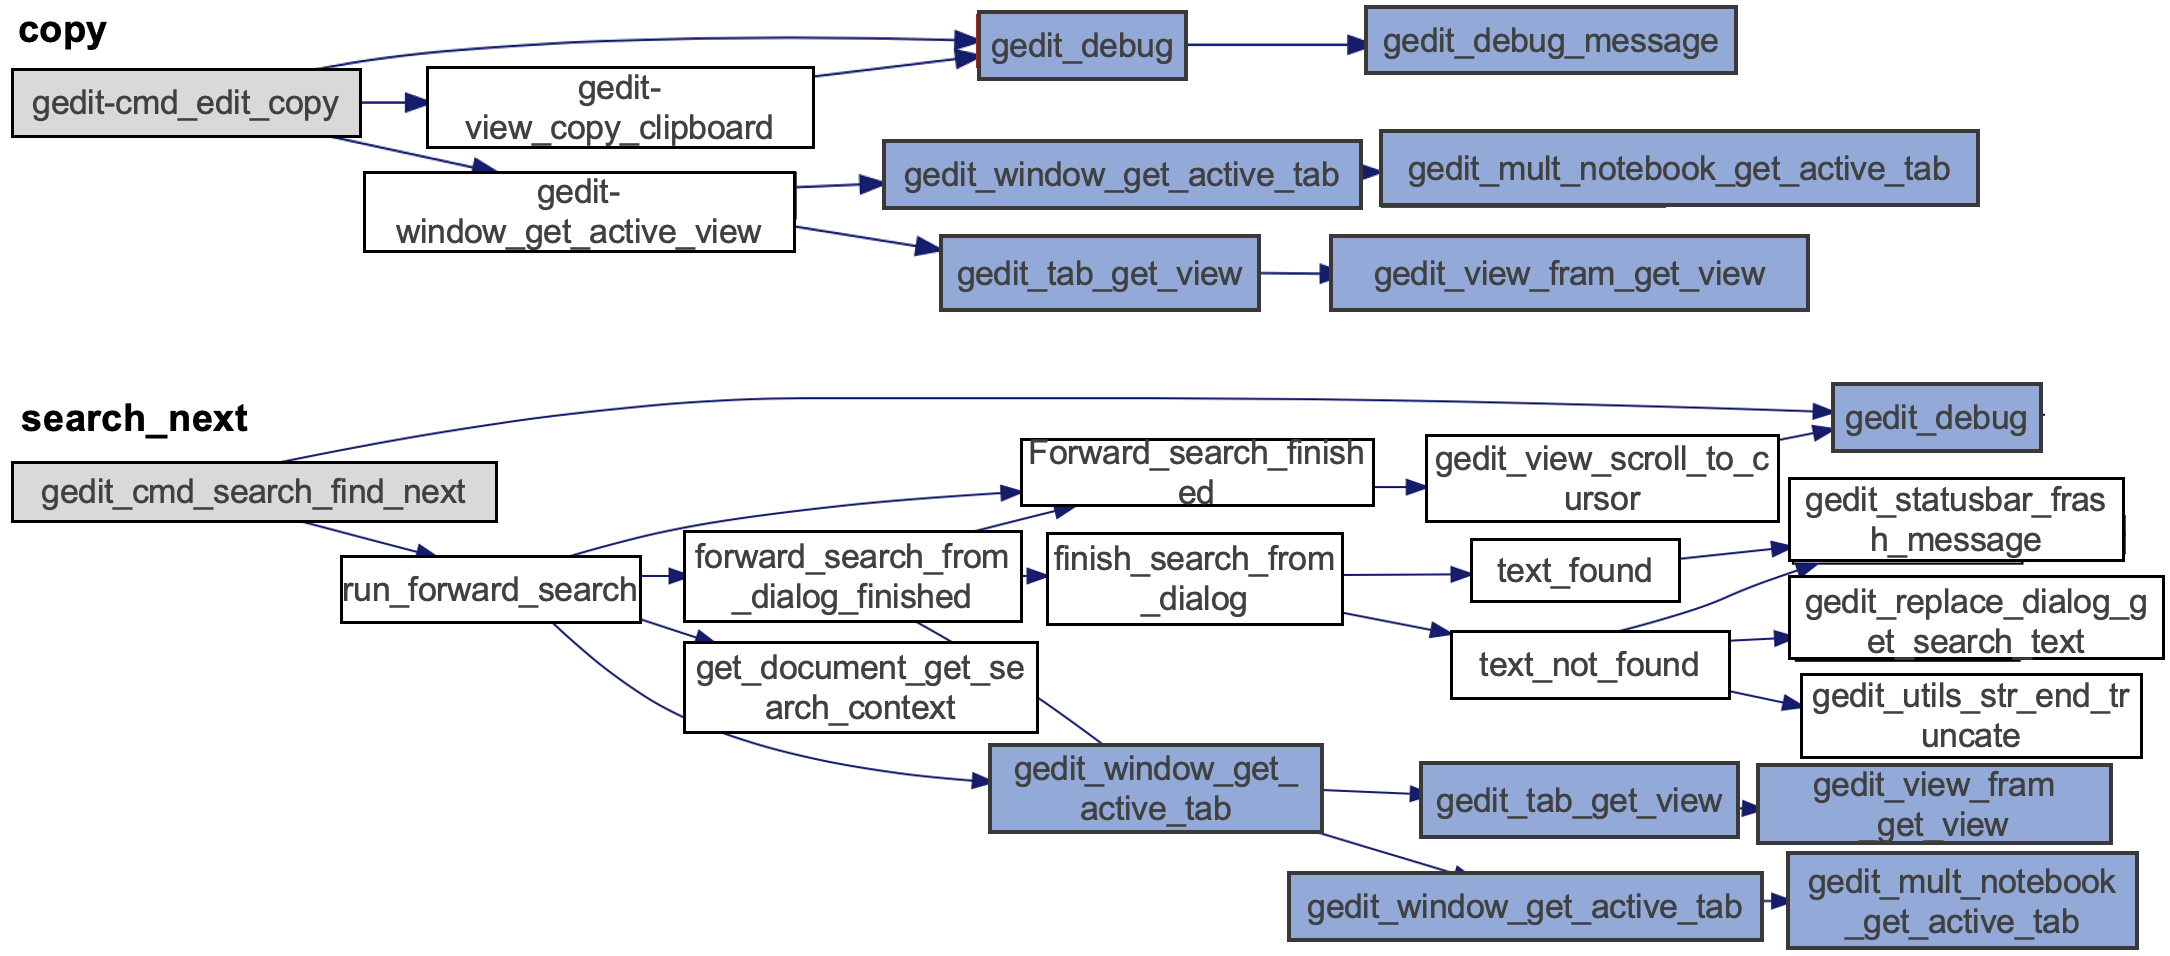
\includegraphics[width=\linewidth]{images/organs_dependency2.png}
	\caption{An example of connection points between the \emph{copy} and \emph{search\_next} organs. Highlighted with red boxes are functions belonging to both organs.}
%	\Description{The 1907 Franklin Model D roadster.}
	\label{fig:organs_connection_point}
\end{figure} 

Although the significant part of these overlaps is pruned from over-organ during GP-refinement, in the source code, one or more program elements within the boundaries of an organ depend on elements external to that organ, such as a function defined in one organ and called by another organ. In other words, organ dependencies are established by means of structural dependencies in the source code shared between elements of different organs~\cite{CafeoA2016}. When this happens, the \emph{organ collision} problem occurs that if it is not managed the transplantation process would add unwanted code duplication.

Thus, we need to do more than merely insert foreign code (self-contained) into the product base without any connections among the organs already transplanted. We need to augment the functionalities of the postoperative product base with new behaviour that replicates the software organ extracted from the donor without generating code duplication in a way that common parts of code may be shared among them.

In our approach, code elements (functions, directives, constants, declarations of several global variables and their definitions) already belonging to the beneficiary or to more than one organ are characterized as \emph{implicit connection points} since they can represent a connection or dependence points among two or more organs. That way, we need to identify these kinds of code elements and insert them one at a time, avoiding code duplication. However, hosts tend to have large input spaces into which \autoscalpel~inserts code. In this way, finding the implicit connection points in the host can be difficult. For instance, functions can have the same namespace but not be identical. Thus, it is necessary to check whether a specific code element is already present in the host, considering not only its namespace but its structure and context at a fine level of granularity to make sure that two portions of code are "clones".

We augmented \autoscalpel with a \emph{code clone detector}, based on NiCad~\cite{Roy2009}.  This clone detector finds exact clones over arbitrary program fragments in the organ and host source code by using Abstract Syntax Trees (AST). Thus, we exploit the benefits of \emph{Program differencing}~\cite{Kernighan1983} technique and TXL~\cite{Cordy2006} to identify and compare potential syntactic code duplication using text-line and ASTs comparison~\cite{Roy2009}

Figure~\ref{fig:code_clone_analysis} illustrates our solution to avoid the organ collision problem. To sum up, the clone detector checks if a specific code element is already present in the beneficiary's environment. Then, the code element is entirely \emph{grafted}, \emph{discarded}, or \emph{merged}. In this last case, \autoscalpel introduces additional line breaks such that potential variances within statements and other structures can be accurately inserted by using sub-abstract tree comparison. 

\begin{figure}[t]
	\centering 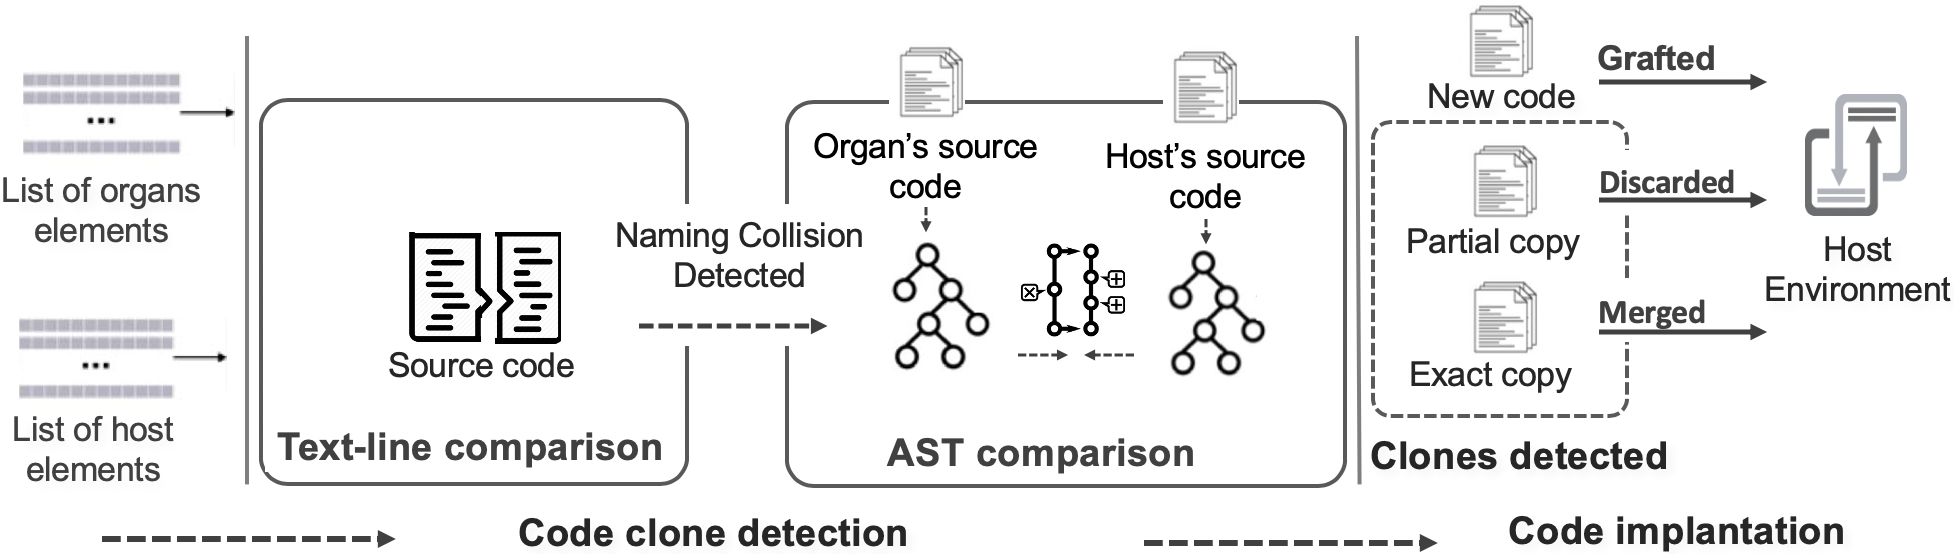
\includegraphics[width=\linewidth]{images/code_clone_analysis.png}
	\caption{Code clone resolution. }
	\label{fig:code_clone_analysis}
\end{figure} 

\subsection{Postoperative Stage} \label{ch:postoperative}

As in medicine, \FOUNDRY requires checking the side-effects of the transplantation operation. For this, we have to perform regression and acceptance testing. 

\FOUNDRY's last stage, its postoperative stage, introduces three validation steps, as outlined in Figure~\ref{fig:postoperative_tests}. Extending the validation process proposed in~\cite{Harman2013, Barr2015}, we highlight the three test suites that \FOUNDRY uses to evaluate the quality of a transplant:  Regression, Regression++, and/or Acceptance.

\FOUNDRY uses the product base's regression tests to check if the transplant does not disrupt the product base's behaviour. Some successful transplants add new functionality to the product base itself;  when that happens, the product base's \emph{regression} test suite must be updated with \emph{regression++} and  \emph{acceptance} tests from each such transplanted organ.

The  host's regression test suite is also manually augmented. Given the transplantation process introduces foreign code into the product base, it is unreasonable to expect its pre-existing test suite to continue to achieve high statement coverage. Hence, to achieve higher coverage, it can be necessary to add new tests to the host's existing test suite by creating regression++; %repetition: , an augmented regression test suite.

An \emph{acceptance} test suite for the postoperative product, manually updated to test the current transplanted functionality at the system level. It checks if the transplanted organ implements the new desired behaviour correctly. 

\begin{figure}[t]
	\centering 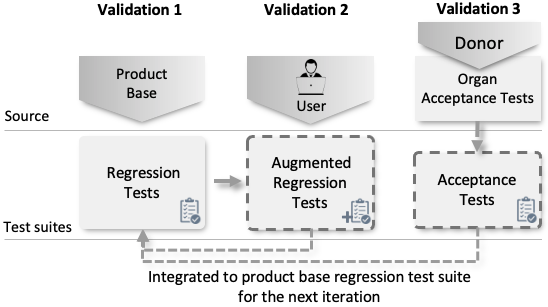
\includegraphics[width=7cm]{images/postoperative_tests2.png}
	\caption{Three validation steps; the dashed boxes are test cases added into the host regression test suite after each transplant iterations.}
	\label{fig:postoperative_tests}
\end{figure} 

Once \autoscalpel has successfully transplanted an organ into the product base, and the result has passed all postoperative validation steps, we incorporate the regression++ and acceptance tests into the host existing regression test suite for use in the next transplantation.

After this stage, new iterations of organ transplantation can be performed; thus, in a stepwise and incremental way, new products are derived as organs are transplanted. This process continues until all organs candidates have been transplanted, and the target product is derived. 

%\section{Implementation Aspects} 
\label{sec:implementation_aspects}

This section presents how the proposed tool was implemented in order to provide a solution for automated the reengineering process of existing systems to SPL. It gives more details about some technical aspects of \autoscalpel tool implementation. Moreover, it presents some challenges found in the implementation process that are enumerated together with the solution implemented.

Implemented in  C and TXL, \autoscalpel comprises 40k SLoCs, of which 23k is C and 17k is TXL code. It requires as inputs for each transplant interaction an organ’s entry point, an insertion point in the host and all C source code and header files in the donor and host's sub-directories. The developer also must supplies test suites that guide the search for donor code modifications required to make it fully executable (and pass all test cases) when deployed in the product base. Given these inputs, \autoscalpel transfer all the code in the donor that implements the target functionality and incrementally produces a new product on a product base. 

The \autoscalpel is an ST tool, which reuses features from multiple systems for transplantation and genetically combines them into one or more product base to attend specific application domains. This is a challenging application of transplantation because code from multiple systems are unlikely to even compile when it is re-located into an unrelated foreign product base without extensive modification, let alone execute and pass test cases. Moreover, the extraction of the code also involves identifying all semantically required code and the successful insertion of the code organ into the host requires nontrivial modifications to the organ to ensure it adds the required features without breaking existing functionality.  

To make this possible, our tool incorporates a set of already consolidated reengineering, search-based and engineering practices into the ST process such as (i) \emph{program slicing} \cite{Binkley:2014:OLP:2635868.2635893} to automate the location; \emph{genetic programming} and (iii) \emph{testing}  to features transformation; and (iv) \emph{code clone detection}, (v) \emph{Program differencing} to handle code duplication and organ collision problems.

To  achieve  the  transplant  of  multiple  organs we had to implement solutions to the new some challenges associated with the necessity to compose multiple organs into a single code base.

\subsection{Handling Preprocessor Directives}

The preprocessor conditionals (cpp) found in large systems often have a set of complex Boolean definitions that encode configuration dependencies, and complex nesting to allow code sharing between configurations. From the maintenance point of view, compile-time configurability brings big challenges~\cite{Tartler2011}. On of them is the necessity of the configuration model (as presented to the user) and the configurability that implemented in the code level have to be kept in sync, which, if performed manually, is a boring and error-prone task~\cite{Tartler2011}. Moreover, once a configuration is defined and a new product is generated, the unnecessary portion of the code (consisting of unselected configurations) can be considered dead code. Thus, ideally would remove dead code, keeping just the code required one by the current system configuration.

\textbf{Solution}. As our proposed is based on construct products on a product base we had to implement a preprocessor directives handler, also used to remove unwanted directives in the organs. This implementation also fix one of the initial algorithm limitation, its default C grammar’s inability to properly handle preprocessor directives. Our solution \autoscalpel uses the command line tool \emph{unifdef}\footnote{http://freshmeat.sourceforge.net/projects/unifdef}  which selectively processes conditional directives. By receiving as input a list of all possible configurations and the guidelines to switch between them, it removes from the donor systems both the directives and the additional text that they delimit, while otherwise leaving the required portion of code defined by the current configuration file, keeping unchanged the source code structure belonging to the organ. 
    
Although useful, only select processes directives is not the best solution, because it does not really understand programming language's lexical and grammatical syntax. For example, \emph{unidef} does not handle defined or \#elif preprocessor directives or handle more complex problems, such as determining that both sides of a conditional assign the same value to a preprocessor variable. To handle this weakness, \autoscalpel has also been implemented in TXL~\cite{Cordy2006}. From it, \autoscalpel becomes able to more reliably remove such dead code and compilation directives, by removing unused configurations.
%============================

\subsection{Multiple-file Slicing} 
    
The extraction of each selected organ captures a considerable amount of code not confined in a single file or library. Thus, an important issue, which must be considered during organ extraction, is how to organize the code belonging to a particular organ in terms of its file structure. Although it is possible to implement modifications to organ's files structure and even introduce a new one, we have chosen to maintain it in its original form, as implemented in its donor, without any redesign of the system besides those ones performed by GP during GP-refinement. This is justified when we consider the inherent complexity of the process, which often decreasing readability and maintainability while introducing the potential for additional programming errors. 

\textbf{Solution}. Program slicing technique implemented in $\mu$scalpel was extended to produce a multi-file organ. We had to implement a multi-file slicer that computes slices in multi-files, keeping the original file structure of the features rather inline all their functions calls in a single file. Thus, each slice constructed includes either the files which each statement has been originally captured, necessary to produces an organ composed by multiple files. Producing a multi-file organ became it more self-contained and more understandable, facilitating future maintenance of the organ in the new product. Additionally, by computing multi-file organs, we avoid code duplication by handling dependencies between organs when transplanted from the same donor.

%=====================
\subsection{Code Duplication} 

As detailed in stage five of our approach description (\ref{organ_implantation}), an organ into a donor program may share common portions of code with other organs. This characteristic creates a high-degree complex interaction which must be considered during autotransplantation process in order to generate a product line without code duplication.

\textbf{Solution}. To automated the comparison of features, we implemented in \autoscalpel a code clone detector based on the \emph{NiCad}~\cite{Roy2009}. We combine \emph{Clone detection} and \emph{Program differencing} techniques for the purpose of comparing features and avoid the code duplication and overlapping of features elements during the implantation process of multiple features. Thus, \autoscalpel can handle feature dependencies using a context-free parsing mechanism implemented in TXL. 

The code clone detection technology provides an intuitive mechanism to include code only when a new element has not been selected in previous organ transplantation. In this case, \autoscalpel checks if there is some element into the organ that is already presented at a list of elements transplanted. Once that potential code duplication is found, it is analysed using program differencing techniques implemented to execute the \emph{GNU DIFF} commands.

The program differencing tool, diff, used to identify individual textual differences at a line level, even that it reflects changes in the organs already transplanted. Thus, \autoscalpel identify what changed between the organ and host code while carrying out peer code reviews, resolving parallel edit conflicts. 

Although useful, this is not enough solution yet, because a line-by-line code comparison does not really understand programming language's lexical and grammatical syntax. For example, \emph{unidef} does not handle more complex problems, such as determining high-level software changes such as refactorings~\cite{Fowler1999}, \cite{Chikofsky1990} and crosscutting modifications~\cite{Kiczales1997} often consist of a group of changes that share similar structural characteristics.

We exploit the benefits of TXL~\cite{Cordy2006} to identify and compare potential syntactic code duplication, as shown in Figure~\ref{fig:code_clone_analysis}. Thus, the clone detector finds exact clones over arbitrary program fragments in organ and host source code by comparing abstract syntax trees. It checks if a specific code element is already present in our beneficiary by looking for \emph{name collisions} in organ and host abstract tree. From this, we may tune the existing code of potential clones to introduce additional line breaks such that potential variances within statements and other structures can be accurately inserted by using sub-abstract tree comparison. 

Our solution complements the feature aggregation process though GP by locating and dependency handling when the reengineering process requires the transplant of two or more features from the same donor. Using a line-by-line and semantic code comparison, we can accurately determine which elements are shared between the organs transplanted, preventing shared elements from being inserted into the host again. 

\subsection{Precise Call Graph Construction}

Call graph construction is an important part of the program slicing process implemented in our solution since it makes the set of functions that may be the target of a given call explicit. For the construction of the call graphs, $\mu$\textsc{scalpel} uses \emph{GNU cflow}, and thus inherit its limitations related to function pointers and such as its stack limit and large output graph production which precludes parsing large programs. If the output graph is large, it can be time-consuming and expensive for TXL programming to construct and manipulate the program. The construction of a more precise call graph more precisely approximates the over-organ to the real organ, at a reduced effort and time to compute, and take up less amount of memory.  
\textbf{Solution}. Unlike initial transplantation tool, \autoscalpel is implemented with a more precise mechanism of call graph generation by using \emph{Doxygen}\cite{Doxygen2018}, a source code documentation generator written in C++. It able the production of individual call graphs which means that for each procedure, the graph contains a separate node for each call stack that procedure can be activated with. This allows the more precise call graph obtainable and individual identification of all program elements relevant to a feature—it fixing one of the initial tool problems such as its stack limit which precludes parsing large programs. 

\subsection{Automatic Organ-host Interface Construction} 

Harman et al.~\cite{Harman2013} proposed that one steps to achieve AST would be the automatic construction of an organ-host interface, responsible for providing access to the organ from and within the host.  In addition to the benefits of encapsulation that this interface can provide, its automatic implementation also frees developers from the burden of writing the code to connect up and convert host data structures into organ parameters. 

\textbf{Solution}. We have introduced an \emph{organ-host converter}.  \autoscalpel inserts a call to this converter at the implantation point in the host. Then, \autoscalpel~constructs an organ-interface which is filled automatically by GP during the organ adaptation process. At the interface, GP tries to bind the parameters at the implantation point with variables in the organ's interface signature. GP synthesizes a call to the extracted organ within the host. The interface constructed will be sufficient to allow the host to access the organ as a component at the code level and that its implementation will be hidden through encapsulation. In addition to the benefits of encapsulation that its interface provides, this converter also frees developers from the labour-intensive task of manually annotating feature entry points. 

%\section{Comparative Study on Automated SPL Reengineering Practices via AST}{} \label{sec:comparative_study}

Many contributions (including industrial experiences) can be found in the reengineering literature~\cite{Assuncao2017}. Nevertheless,  there is a lack of automated approaches covering the whole life cycle of reengineering for a product line~\cite{Assuncao2017}. The most of existing solutions are responsible for the dependency on expert knowledge, manual labour or by using a combination of multiples tools, which is one of the reasons why the reengineering process is still a laborious, time-consuming, and error-prone task that requires a high upfront investment before the first product is produced from an SPL\cite{Krueger2001, Bastos2017, Assuncao2017}. 

We argue that ST can be a feasible technique for migrating existing systems to product lines. However, to be able to explore it as a promising new research direction with application in reengineering for SPL, we need to compare it with existing practices regarding its support to the reengineering process and limitations. 

In this sense, we conducted a comparative study in the existing literature to evaluate the feasibility of using the approach from the analyse of: (i) how software transplantation supports SPL reengineering phases, and (ii) how it provides a solution for addressing SPL reengineering open issues in comparison with the existing solutions.

The remained of this chapter consists of four sections. \textbf{Section \ref{sec-ch5:exploratory_study}} introduces the exploratory study goal and research questions. \textbf{Section \ref{sec-ch5:spl_reengineering}} gives an overview on existing approaches and main open issues. \textbf{Section \ref{sec-ch5:discussion}} discusses the analysis of the study and threats to validity. \textbf{Section \ref{sec-ch5:conclusion}} draws concluding remarks and points out future directions. 

\section{The Comparative Study} \label{sec-ch5:exploratory_study}
This section presents the design, objectives, research questions and selection criteria considered in our comparative study.

Assunção et al.~\cite{Assuncao2017} described many open issues on SPL reengineering research including the following: (i) the implementation of automation and tool support, (ii) the use of different sources of information, (iii) need for improvements in the feature management, (iv) the definition of ways to combine different strategies and methods, (v) lack of sophisticated refactoring, (vi) need for new metrics and (vii) measures and more robust empirical evaluation~\cite{Assuncao2017}.

In order to demonstrate the potential to use autotransplantation as an automated solution to address the open issues, we compare it with the current reengineering practices for extracting an SPL from existing code bases. 

This investigation can support our proposal as it allows us to better understanding and demonstrates some evidence of how AutoST can be a feasible solution for SPL reengineering projects. We acknowledge the importance of new studies to compare our tool with other solutions using real-world systems in the evaluation what would make it possible to compare the reengineering process and the resulting product line. However,  a common issue is the lack of a framework for comparing reengineering approaches~\cite{Assuncao2017}, mainly that can deal with the reengineering of systems implemented in C as supported by our tool.

\subsection{Objective and Research Questions}

The objective of this study is to analyse and discuss our proposal in comparison with the current practices in the field of reengineering of systems into SPL, thereby demonstrating the potential of autotransplantation technique for addressing existing open issues. Thus, the following questions were established:

\begin{itemize}
    \item \textbf{RQ1.} \emph{How does multi-organ transplantation (as realised in \FOUNDRY) automate existing reengineering practices for extracting an SPL from a codebase?} Already exist a set of tools~\cite{Assuncao2017} that supports reengineering of systems variants into SPL which are used to produces code refactored. To demonstrate that a new solution can evolve the current state of practices of the reengineering to obtain an SPL cannot be easily answered without a comparative analysis among the existing solutions. Thus, we used the reengineering approaches existing in the literature to answer our first research question. We selected a set of approaches that also propose automated solutions for SPL reengineering process and produce source code refactored as output. 

    \item \textbf{RQ2.} \emph{Do the transplantation approach for obtaining SPL address any of the open issues in the field of reengineering of systems variants into SPL? If so, how does it address such challenges?} It is important to understand if AutoST implements any solutions to the open issues identified by ~\cite{Assuncao2017}. This question aims at analyzing what/how the current limitation of the existing solutions can be addressed by our approach. 
\end{itemize}

\subsection{Selection Criteria}

Our main source of information was the systematic mapping performed by Assunção et al.~\cite{Assuncao2017}. According to the authors, from the total of 119 existing studies for guiding the SPL reengineering process, only 19 of them the authors provide automated support to their methods, considering tools that are specific for the reengineering process.

Many proposed tools have focus on more than one phase. Nevertheless, most part of them only covers the \emph{detection} and \emph{analysis} phases (8), \emph{Variability to Aspect tool}~\cite{Alves2007}, \emph{CoDEx Tool}~\cite{Trifu2010}, \emph{FeatureMapper}~\cite{Heidenreich2008,Seidl2012}, \emph{MapHist Tool}~\cite{Nunes2014}, \emph{ExtractorPL}~\cite{Ziadi2012}, \emph{AUFM Suite}~\cite{Bagheri2011}, \emph{FMr-T}~\cite{Mazoun2014}, \emph{ArborCraft}~\cite{Weston2009}; followed by one (1) that gives support only to the analysis phase, \emph{ETHOM} ~\cite{Nunes2012}; and \emph{Model Driven SaaS}~\cite{Mohamed2014} tool that provides support only to the \emph{transformation} phase (1). Thus, a total of eight (8) remaining tools cover both three phases, \emph{ThreeVaMar}
~\cite{Rubin2010}, \emph{Recfeat}~\cite{Nunes2012}, \emph{Clone-Different}~\cite{Xue2011}, \emph{SPLevo}~\cite{Klatt2014}, \emph{Theme/SPL}~\cite{Araujo2013} \emph{BUT4Reuse}~\cite{Martinez2014}, \emph{ECCO Tool}~\cite{Fischer2015}, \emph{JfeTkit}~\cite{Tang2015}. 

It is important to observe that the transformation phase allows the actual systematic reuse of the artefacts, and source code refactored is the most common outputs~\cite{Assuncao2017}. Source code refactored is an output provided to allow a better organization of the features with the SPLE. Thus, in order to select the most relevant set of tools regarding its support of the entire process of reengineering and eliminate studies which do not address the research questions, the following criteria were used to form the final set of tools included:

\begin{enumerate}
    \item The tool must cover all phases of the reengineering process, i.e., detection, analysis and transformation;
    \item The proposed tool  must produce source code refactored as output; and
    \item Tool considering code as input artefact. 
\end{enumerate}

Finally, a total of six remaining tools were selected based on these criteria and compared with our proposal. We analyzed the selected tools by looking at its publication, their documentation such as development documents and user manuals, and available extensions (such as plugins) in those tools which have an extensible architecture.

\section{Tool Support for Reengineering of Systems into SPL} \label{sec-ch5:spl_reengineering}

The main reason to provide automated support to the reengineering process is to reduce the manual effort~\cite{Martinez2014, Abbasi2014}. Moreover, an automated process can improve the overall quality of the reengineering process since this process is a labour-intensive task and error-prone~\cite{Stoermer2001}.  In this sense, authors argue for the necessity of providing tool support, such as~\cite{Sampath2014, Passos2013, Zhang2011, Acher2013}. However,  in many cases, the reengineering researchers expose only an intention to provide an automated solution to their methods~\cite{Assuncao2017}. Further studies should envisage the implementation of tools to automate to support the entire reengineering process. 

We present a summary of the tools selected and analysed in this study that were used for our approach evaluation. A brief description of the tools and corresponding work references are presented below:

\begin{itemize}
    \item \textbf{Recfeat~\cite{Nunes2012}}: a prototype tool developed to support the use of the history-sensitive heuristics for the recovery of features in code of degenerate program families. RecFeat tool is used to classify the features’ code elements of the selected program families. Once the analysis of the family history is carried out, the feature elements are structured as Java project packages; they are intended to separate those elements in terms of their variability degree;
    
    \item \textbf{Clone-Different~\cite{Xue2011}}: a Clone Differentiator tool that automatically characterizes clones returned by a clone detector by differentiating \emph{Program Dependence Graph} of clones. The tool complements clone detection with semantic differencing of reported clones. It is able to provide a precise characterization of semantic differences of clones.

    \item \textbf{SPLevo~\cite{Klatt2014}}: a software development tool that supports the consolidation of customized product copies into a SPL based on program dependencies as represented in \emph{Program dependency graphs}. It reduces the effort of consolidating developers when identifying dependent differences and deriving clusters to consider in their variability design; 
    
    \item \textbf{BUT4Reuse~\cite{Martinez2014}}: (Bottom-Up Technologies for Reuse) a tool-supported bottom-up SPL adoption framework specially designed for genericity and extensibility. This tool provides technologies for leveraging commonality and variability of software artefacts.

    \item \textbf{ECCO Tool~\cite{Fischer2015}}: (Extraction and Composition for Clone-and-Own) automatically locates reusable parts in existing systems and compose a new system from a selection of desired features. It gives support to an approach to enhance clone-and-own that supports the development and maintenance of software product variants. By following this approach, a software engineer selects the desired features, and ECCO finds the proper software artefacts to reuse and then provides guidance during the manual completion by hinting which software artefacts may need adaptation; 
    
    \item \textbf{JfeTkit~\cite{Tang2015}}: (Java Feature Mining Toolkit) extracts featured code from the software legacy. JFeTkit is a compound system, which uses several existing software analysis libraries, including BCEL (Byte Code Engineering Library), Crystal3 analysis framework and JDT (Java Development Toolkit). JFeTkit collects the information generated using these third-party APIs and annotates software code legacy using a top-down feature mining framework by for SPL proposed in~\cite{Tang2015}.

\end{itemize}

\section{Results and Discussion} \label{sec-ch5:discussion}

Even with numerous researches and advancements, open issues remain in the field of reengineering (with focus on SPL). Assunção et al.~\cite{Assuncao2017} identified these research gaps and limitations. From these, they reported the research opportunities and trends uncovered. To answer both of our research questions, we analysed which open issues existing in reengineering practices are addressed by existing tools and compare them with the solution implemented in \autoscalpel using ST technique. We summarize the results in Table~\ref{tab:comparison_issues}.

\begin{table*}[t] 
	\caption{Comparison of the \autoscalpel~with existing reengineering solutions to SPL regarding the strategies used and open issues addressed based on~\cite{Assuncao2017}.
	}
	\label{tab:comparison_issues}
%	\resizebox{\columnwidth}{!}{%
		\begin{tabular}{lcccccccccccccccccccc}\\\hline
		%\toprule
			Tool & \multicolumn{5}{c}{Strategies} 
			&& \multicolumn{4}{c}{Input} && \multicolumn{8}{c}{Open Issues}\\
			\cline{2-6} \cline{8-11} \cline{13-20}
			&Exp. &Stat. & Dyn. & IR & SB &&
			Test & Req.  & Des. & Code. & &
			1 & 2 & 3 & 4  & 5 & 6 & 7 & 8
			\\\hline
		   	\rowcolor[gray]{.9} 
		   	Recfeat & & \checkmark & & && & & & &\checkmark & && &&&&&&\checkmark\\
			Clone-Different & & & &\checkmark &&&&\checkmark &\checkmark &\checkmark & & &\checkmark  &\checkmark &  &\checkmark &&\checkmark&\checkmark\\
			\rowcolor[gray]{.9} 
			SPLevo & & \checkmark &\checkmark  & & & & & & &\checkmark & &&&&\checkmark&&&&\checkmark\\
		    BUT4Reuse &\checkmark &\checkmark & & & & &  &\checkmark &\checkmark & \checkmark  && &\checkmark& &\checkmark &\checkmark &\checkmark &&\checkmark \\
			\rowcolor[gray]{.9} 
			ECCO &\checkmark &\checkmark & & & & & & &\checkmark & & & & \checkmark & &\checkmark & &\checkmark &&\\
			JfeTkit & &\checkmark & & & & &  & & &\checkmark  &&&&&&&\checkmark&\checkmark &\checkmark \\\hline 
			\rowcolor[gray]{.9} 
			\autoscalpel  & & &\checkmark & &\checkmark & &\checkmark & &  &\checkmark & &\checkmark&\checkmark&\checkmark&\checkmark&\checkmark&\checkmark&\checkmark&\checkmark\\\hline 
		\end{tabular}
%	}
\end{table*}

Open issues:

\begin{enumerate}
    \item \emph{Automation and tool support.} The first reason to provide tool support for the reengineering process is to reduce the manual effort~\cite{Martinez2014, Abbasi2014}. Despite the need to automate the entire reengineering process, existing solutions provide support for specific tasks, still requiring manual effort. Additionally, Assunção et al.~\cite{Assuncao2017} highlighted that there is still no tool for feature aggregation and abstraction. \autoscalpel~was implemented to be an automated solution for analysis, detection and transformation tasks, including with automated support for feature aggregation using GP and clone detection techniques. Our solution automates the process of feature location and dependency handling when the reengineering process requires the transplant of two or more features from the same donor.
    
    \item \emph{Exploiting multiple sources of information for reengineering}. Another research gap is exploiting different information sources during the reengineering process. For example, a research opportunity is using test cases, commonly available in most projects, in conjunction with other sources to determine features~\cite{Knodel2005}. Many studies generate feature models as output but, in general, constraints, such as one feature requires or excludes another feature, are not considered~\cite{Assuncao2017}.  Two of the existing tools use more than one source, \emph{Clone-Different} and \emph{BUT4Reuse}. Our ST solution uses source code as input, but the process feature extraction is also guided by test suite observation.
    
    \item \emph{Feature  management.} Feature management is an important task in the reengineering process, responsible for providing variability among the features that compose the product variants. Many studies generate feature models as output but, in general, constraints, such as one feature requires or excludes another feature, are not considered~\cite{Assuncao2017}. \autoscalpel~provides partial support to this task by dealing with dependencies and interactions among features at code level using clone detection.
    
    \item \emph{Hybrid Approaches.} Hybrid approaches can improve the results when compared with the application of only one type of strategy~\cite{Assuncao2017}. The combination of techniques is one of the main characteristics of our solution. Regarding the selected solutions, only \emph{SPLevo} consider the combination of dynamic and static analysis strategies. There is still no tool for that consider search-based techniques as a strategy to reengineering process. \autoscalpel~has been implemented to extract and transform features using a form of dynamic observational strategy, close to dynamic analysis, in combination with GP. 
    
    \item \emph{Refactoring techniques.} Assunção et al.~\cite{Assuncao2017} highlighted the need for new refactoring techniques. The Search-based strategy, for example, has been little explored in the area of SPL~\cite{Lopez2015} and has the potential to exploit as a combination of different strategies~\cite{Harman2014a}. Regarding new refactoring techniques, our solution explores ST as a new approach to obtain SPL.Regarding the transformation phase, Olszak and Jørgensen point out the labour-intensive task of manually annotating feature entry points~\cite{Olszak2012}. Full automation of the process has been considered unrealistic due to the complexity of the task~\cite{Biggerstaff1993, Kastner2011, Lopez2011}. Even that existing techniques for locating a feature’s implementation~\cite{Harman2002,Komondoor2000,Lanubile1997}, domain experts still need to confirm whether found code fragments belong to the feature and then adapt it to the product line~\cite{Kastner2011}. 
    
    \item \emph{Need of usage guidelines.} Many authors argue the necessity of the creation of guidelines to formalize the tasks of their proposed approaches~\cite{Assuncao2017}. In a similar way,  Kang et al. point out the need for guidelines for evaluating product line assets~\cite{Kang2005}. Half of the solutions selected propose some kind of guideline that formalize the tasks predict in their proposed approaches. \FOUNDRY provides a detailed guideline for automating the extractive SPL reengineering process. Such guideline can, with suitable tailoring, be applied in a wide range of projects and domains. Additionally, \FOUNDRY~predicts three validation tasks that together can provide a suitable form to validate the productized products.

   \item \emph{New Measures and Metrics.} Measures and metrics are important for the reengineering process~\cite{Assuncao2017}. Nöbauer et al.~\cite{Nobauer2014}, for example, exposed the need of a similarity calculation method that allows the identification of commonalities among existing products. \FOUNDRY does not provide support to measure and metric with similarity calculation method to identify commonalities in existing products. However, this gap is minimized by using ST, and a clone detection approach to productize software and deal with eventual dependencies among the features transplanted from different systems.

    \item \emph{More Robust Empirical Evaluation.} Researchers acknowledge the importance of using real case studies. However, the most of authors of tooling support for SPL reengineering expose only an intention to provide empirical evaluation using their approaches in different domains and with complex case studies are~\cite{Assuncao2017}. The great majority of the researchers provide some kind of evaluation of their solutions. In some cases, their creators acknowledge the necessity to perform more evaluation using real case studies. On the other hand, we conducted two case studies that deal with relatively large systems and provide plausible real-world scenarios. Nevertheless, we also acknowledge the importance of more studies using real-world scenarios to validate the scalability and feasibility of the ST process for SPL reengineering. 
    
\end{enumerate}
In summary, although approaches to conducting the reengineering process with a focus on SPL have been proposed \cite{Assuncao2017}, they provide incomplete solutions to transform those single products into an SPL by focusing on part of the process \cite{Assuncao2017}. Many approaches lack the means to consolidate different features present in more than one product, other has not automated support to the phases of the process, or fail by not exploiting multiple sources of code for reengineering \cite{Assuncao2017}. Moreover, the existing solution~\cite{Fischer2015} only cover the reuse of variants from related systems or from the same family what limit the potential of existing codebases reuses for SPL. On the other hand, AutoST for SPL reengineering emerges as an ambitious initiative that could, in the future, makes possible the reengineering among systems even from different languages and platform. 

We believe that with more research and suitable tailoring, AutoST approach can make the reuse of one or more products to generate a new one possible by transplanting features from pre-existing systems. Open source projects, for example, can enable every developer the opportunity to share codes, allowing them to migrate an already existing code from a pre-existing source to their own SPL project. In the same way, software organisations could derive new software products from its existing systems portfolio.

\section{Case Studies} \label{sec:case_studies}
We evaluate \autoscalpel~on two case studies for generating new product variants from real-world systems. This section explains the objectives, research questions, and subject systems. Additionally, it presents the results of our study and discusses the implications.
%%%%[Extracting product lines from variants (explant)]In an automated process, developers can then derive a software product from the software platform and the given configuration.
%Incremental Integration. We conducted case studies on analyzing legacy systems [16], extracting software product lines [17, 20], and combining variability mechanisms [18]. A particular result of these studies are defined processes for developing features and migrating source code. Our

\subsection{Objective and Research Questions}
The objective of this study is to evaluate the proposed approach and tool, thereby demonstrating the potential of automated software transplantation for product line generation. % and 
We aim to answer the following research questions:

\textbf{RQ1.} \emph{How much effort is required to generate products from a product line created using \autoscalpel?}

Given the complexity of the task at hand, it seems unreasonable to expect the product derivation process to be instantaneous. Still, it will need to be fast enough to be incorporated into a development cycle and demonstrate its advantage with regard to manual effort. To answer this question, we computed the time required, and the number LoCs transferred to productize software.

\textbf{RQ2.} \emph{How many features could \autoscalpel~productize?}

We discuss the characteristics of features that \autoscalpel~can and those it cannot yet handle. Given the inherent complexity of the process, it is important to clearly define its current limitations. 

We answer our first two research questions by simulating two transplantation scenarios. In the first scenario, we used \autoscalpel~to derive a small text editor, \emph{Product A}, using a reduced version of \emph{VI} as our product base. In the second scenario, we derive \emph{Product B}, a more significant text editor (in terms of the number of code lines and functionalities), using VIM as raw material for the product base. We used as donors four real-world systems in both scenarios.

\subsection{Subject Systems}

We chose subjects of two different domains and with a wide range of sizes in order to remove bias regarding specific properties of a particular application domain. However, we included three text editors to account for different coding styles within a single domain. Such choice was important to give evidence that \autoscalpel~can also be used to achieve a product line from a distinct set of usage scenarios. 
Presented in Table~\ref{tab:donors_list}, our donors include three text editors, \emph{kilo}, \emph{VI} and \emph{VI}; and \emph{GNU Cflow}, a call graph extractor from C source code. We identified the following features as possible desired features in a new editor: $\texttt{output}$ from CFLOW, $\texttt{enableRawMode}$ from kilo, $\textt{vclear}$ from VI, and $\texttt{spell\_check}$ and $\texttt{search}$ from VIM. Table~\ref{tab:donors_list} gives more details on the subjects.

\begin{table}[t]
\centering \small
	\caption{Donors and hosts corpus for the evaluation: column Features shows the number of features identified. 
	}
	\label{tab:donors_list}
	\begin{tabular}{llrr} \hline
        Subjects &Type  & Size (LoC) & \#Features   \\\hline
	    Kilo     &Donor & 804        & 17      \\
		CFLOW    &Donor & 4,274      & 54      \\
		VI       &Donor & 20,292     & 36      \\
		VIM      &Donor & 839,438    & 176      \\\hline
		VI       &Product Base & 20,223 & 36      \\
		VIM      &Product Base & 737,466 & 117     \\\hline
	\end{tabular}
\end{table}

\subsection{Results and Discussion} \label{sec:result_discussion}

Each organ transplantation was repeated 20 times, as the underlying algorithm, which is based on GP, is stochastic. The runtimes for each transplantation were measured on an Intel Core 3.1 GHz Dual-Core Intel Core i5, with 16 GB memory running MacOS 10.15.4.
  
Table~\ref{tab:transplantation_time} shows average timings of transplanting each organ into the product base as well as the total number of code lines transplanted to derive each product. At the end of the transplantation process, the postoperative product A has a total of 28k LoC and 40 features while product B has a total of 745k LOC and 121 features. Together, donors provided three feature variants to the product line, approximately 7.8k LOC to product A and 8.1k to product B, including a feature removed and re-transplant in \emph{VI}

\begin{table}[t]\centering \small

%	\resizebox{12cm}{!}{%
    \caption{Multi-organ transplantation results to generate products A and B. \emph{Columns Trans. Time shows the time (Sys+User) spent on the organ transplant process in which column Sys. correspond to the \autoscalpel's execution time; column User correspond to the user time spent in preoperative stage and  augmenting the host’s regression test suite (regression++).}}
    \label{tab:transplantation_time}
	\begin{center}
	\begin{tabular}{lrrrrrr} \hline
		\multicolumn{1}{c}{Donors} & \multicolumn{3}{c}{Number of}   & &\multicolumn{2}{c}{Trans.time(min)} \\
		\cline{2-4} \cline{6-7}
		 & \multicolumn{1}{c}{LoC}  & \multicolumn{1}{c}{Functions} & \multicolumn{1}{c}{Files} & & \multicolumn{1}{c}{Sys.} & \multicolumn{1}{c}{User}\\\hline
	%	MYTAR       &4 & \sim197 & 8 & 8 &  & 74 & 82\\
		Kilo        & 963 & 35 & 4 & & 86 & 32\\
		CFLOW       & 4,822 & 37 & 8 &  & 344 &123 \\
		VI          & 1,983 & 5 & 15 &  & 1234 &184\\\hline
		\rowcolor[gray]{.9} Product A  &7,768 & 77 & 27 & & 1,664 & 339 \\\hline
	%	MYTAR       &4 & \sim215 & 8 & 8 & & 74 & 82\\
		Kilo        & 981 & 35 & 4 & & 94 & 32\\
		CFLOW       & 4,898 & 37 & 8 &  & 428 & 123\\
		VI          & 2,234 & 5 & 15 &  & 1294 & 184\\\hline
		\rowcolor[gray]{.9} Product B  & 8,113 & 77 & 27 & & 1,890 &532\\\hline
	\end{tabular}
	\end{center}
	
    %}	
\end{table}

\begin{framed}
\noindent To answer \textbf{RQ1}, we created two new products by using \autoscalpel. On average, it required 4h31min/1KLoC for transplanting all three features into product A, and 4h40min/1KLOC for transplanting features into product B.
\end{framed}

To answer question \textbf{RQ2}, we tried to transplant two more features:  $\texttt{spell\_check}$ and $\texttt{search}$, both from the largest donor program, i.e., VIM. This effort exposed some limitations of the technologies used by \autoscalpel. The tool inherits the limitations of TXL, such as its stack limit which precludes parsing large programs.

\autoscalpel~also inherits the limitation of generating an imprecise call graph when dealing with function pointers in donor systems. This restriction comes from Doxygen~\cite{Doxygen2018}, a source code documentation generator, used by \autoscalpel~ to generate the call and caller graphs. Function pointers enable indirect memory access through indirect procedure calls. Such indirect calls can be disambiguated with pointer analysis, resulting in an imprecise construction of the program's call graph~\cite{Milanova2004}.  Imprecise call graph can produce a significant impact on donor call graph construction and consequently in the organ slicing process. Although a significant part of sliced over-organ is pruned, during GP-refinement, it continues retaining unnecessary instructions.

Although possible with an additional manual effort, such limitations made our tool unable to automatically extract those organs from a large program like VIM, because they contain indirect procedure calls. We can, in the future, turn to \emph{Dynamic analysis}~\cite{Cornelissen2009} and other code manipulating tools to optimise the efficiency of the slicing process, to efficiently identify those statements in the program slice which have influence on the target organ. 

In summary, these case studies show initial evidence that software transplantation can be successfully used for building product variants automatically by compositing of features transplanted from real-world systems. New studies may give more evidence that our approach is also extensible and flexible in other domains (opening perspectives for new work).

\begin{framed}
\noindent To answer \textbf{RQ2}, \autoscalpel was able to productise three features from three different systems. The tool inherits the limitations of its underlying tools: TXL's stack limit, restricting the size of software parsed; and Doxygen's imprecise call graph generation, possibly retaining unnecessary instructions in the target organs.
\end{framed}
%\section{Experiment} \label{sec:evaluation}
%\subsection{Human Study} \label{sec:evaluation}
\section{Experimental Evaluation} \label{sec:evaluation}

In the previous case study, we showed the viability of our software transplantation approach, implemented in \autoscalpel, to generate software product lines from the existing codebase. Although the validation of the approach is based on empirical evidence, it  is  still important to test its efficiency by comparing it with other tools used to product line migration. Unfortunately, tool support for the reengineering process is limited, in general, they give support for specific activities, such as feature location, refactoring or quality assurance~\cite{Assuncao2017,Kruger2020}. To the best of our knowledge, there is currently no comparable tool that manages to transplant features from distinct donors systems written in C to generate a product line, remaining to us analysing it concerning to human effort. Thus, we conducted an experiment based on Wohlin et al.~\cite{Wohlin2012}, that reflects a real-world process of product line migration from existing codebases ~\cite{Krueger2002}. In this section, we state our research objectives and describe in detail the experimental setting.

\subsection{Goal}
The goal of this experiment is to analyse the effectiveness and efficiency of our approach compared with the manual process of generating a product line from existing systems, performed by SPL  experts. In accordance with the guidelines for reporting software engineering experiments presented in ~\cite{Wohlin2012b}, we have framed our research objectives using the Goal Question Metric (GQM) method suggested by Basili~\cite{Basili1994}. Our goal is to:

\textbf{Analyse} of a software transplantation approach to derive product variants 
\textbf{for the purpose of} comparison 
\textbf{with respect to} effectiveness and efficiency 
\textbf{from the point of view of} the researcher
\textbf{in the context of} an SPL project of product line migration from real-world systems.

\subsection{Research Questions}

In order to achieve the stated goal, we defined two quantitative questions. These are related to the data collected during the period that the experiment was executed. The questions are described as follows:

\textbf{RQ1.} \emph{What is the accuracy of the proposed approach for automated migration of target features to a product line?} In this respect, we would like to understand how accurate our approach is when automatically transferring all required code so that the target feature can run in an emergent product line compared to the manual process.

\textbf{RQ2.} \emph{How much feature migration time can be gained using \autoscalpel compared to the manual process?} With this question, we evaluate the time spent by SPL experts to \emph{extract}, \emph{adapt} and \emph{merge} features to derive new product variants in comparison with the same process using \autoscalpel. 

\subsection{Metrics}
With the objective to answer the previous questions, we defined the metrics that must be computed. For each question, it was defined one metric. These are described as follow:

\textbf{M1.} For the first question, the accuracy of our approach is computed by verifying if \autoscalpel successfully migrated new functionalities to a product line and it passed in all the regression, augmented regression and acceptance test suites. Together, these our test suites check whether or not the output of the transplanted feature is correct with respect 


%[Type Migration in Ultra-Large-Scale Codebases] For this corpus, we provide T2R with TRANSFORMATION SPECIFICATIONS to migrate seven generic Functional Inter- faces to 35 specialized alternatives. We use this corpus to assess the accuracy and usefulness of our approach (i.e., RQ1 and RQ2). Although

%Using the RefactoringMiner API, we obtain the pairs of program elements (i.e., type, method and field declarations), which have been matched between the currently analyzed commit and its parent in the directed acyclic graph that models the commit history of git-based version control repositories. The pairs of matched program elements may have identical signatures (e.g., a pair of methods with identical names, pa- rameter and return types), or may have different signatures due to refactoring operations (e.g., RENAME METHOD, CHANGE PARAMETER TYPE, ADD/DELETE PARAMETER). Java annotations are used in three different form

%Analysing each feature code successful transfered by the subjects to extract a set of common  applications that produces the delta between the commits.

%For the first question, the accuracy of our approach is computed by verifying if \autoscalpel successfully migrating new functionalities to the product line and it passed in all the regression, augmented regression and acceptance test suites. Second, analysis if the code that was automatically transplanted to the host environment is one of the selected by the SPL experts. To be more precise, if we run our approach to automatically assign a set of 100 code lines and, as a result, 70 of these code lines were correctly selected by the SPL experts, then the approach has an accuracy of 70\%. It is important to observe that different code lines can be eventually selected by different experts; however, for the purpose of the metric M1, the transplanted feature must pass at the test suite. 

%We study how frequently developers change test annotations. To provide some comparative statistics, we show the prevalence of test annotation changes compared to common source code transformations (i.e., renames and type changes) at the same program element level (i.e., class, method and field declaration). In particular, we compare test annotation changes at the method level with Rename Method and Change Return Type, at field level with Rename Field and Change Field Type, and at the class level with Rename Class. Such a comparison is attainable because all compared changes are performed on the same kind of program elements. We

%T2R generated 130 patches, out of which 126 compiled and passed the tests successfully with an overall precision of 97%.
 
\textbf{M2.} For the second question, it is simply tracked down the time that is spent with the activities to transfer the target features. Examples of these activities are \emph{code extraction}, \emph{adaptation}, and \emph{merging}. The time for each of these activities was individually collected.

\subsection{Instrumentation}


According to Wohlin et al.~\cite{Wohlin2012}, the instruments for an experiment are classified in objects, guidelines, and measurement. The object instruments of the experiment are two donor systems: \emph{NEATVI}\footnote{https://github.com/aligrudi/neatvi}, vi/ex editor for editing bidirectional UTF-8 text and \emph{Mytar}\footnote{https://github.com/spektom/mytar}, an archive manager besides another version of \emph{NEATVI} used as product base are used in this experiment. 

Manually inspecting the code to transfer a feature to a product line is hard, slow, and possibly a tedious work~\cite{Mahmood2021}. Thus, we chose to select small codebases to avoid participant's tired, in another way, it would the experiment would require too much time of execution. 

Table~\ref{tab:instrumentation} gives more details about the object instruments used in this experiment. These objects were available to download together with a script to automatic setup of the environment.  

%%%%We assume that inspecting the code to transfer a feature to a product line is hard, slow, and possibly a tedious work. Thus, we preferred this way to avoid participant's tired, in another way, it would require too much time of execution. These objects were available to download together with a script to automatic setup of the environment. 

%%According to Wohlin et al.~\cite{Wohlin2012}, the instruments for an experiment are classified in objects, guidelines, and measurement. The object instruments of the experiment are two donor systems: \emph{NEATVI}\footnote{https://github.com/aligrudi/neatvi}, vi/ex editor for editing bidirectional UTF-8 text with 7,114 LoC and \emph{Mytar}\footnote{https://github.com/spektom/mytar}, an archive manager with 1,046 LoC besides a host product base generated from \emph{NEATVI} Small systems are used in this experiment in place of the systems presented in last study. We assume that inspecting the code to transfer a feature to a product line is hard, slow, and possibly a tedious work. Thus, we preferred this way to avoid participant's tired, in another way, it would require too much time of execution. These objects were available to download together with a script to automatic setup of the environment. 

%\begin{table}[t]
%\centering \small
%	\caption{Experiment Design}
%	\label{tab:experiment_design}
%	\begin{tabular}{lll}  \\\hline
%		  & \multicolumn{2}{c}{Instrumentation} \\ 	\cline{2-3}
%		\multicolumn{1}{c}{Scenarios} & \multicolumn{1}{c}{Donor} & \multicolumn{1}{c}{Host}        \\\hline
%		I    & MYTAR & Product base  \\
%		II   & NEATVI & Product base \\\hline
%	\end{tabular}
%\end{table}


\begin{table}[t]
	\caption{Experiment instrumentation}
	\label{tab:instrumentation}
    \begin{adjustbox}{width=\columnwidth,center}
    	\begin{tabular}{l|lr|lr|lr} \hline
    		\multicolumn{1}{c}{Scenario} & \multicolumn{1}{|c}{Donors} & \multicolumn{1}{c|}{LoC}   & \multicolumn{1}{c}{Target features}       & \multicolumn{1}{c|}{LoC}  & \multicolumn{1}{c}{Host}& \multicolumn{1}{c}{LoC} \\\hline
    		I       & NEATVI & 5,276 & $\texttt{DIR\_INIT}$  & 239&\multirow{2}{*}{Product base}&\multirow{2}{*}{5,285} \\
    		II      & Mytar  & 1,046 & $\texttt{WRITE\_ARCHIVE}$ & 170&& \\\hline
    	\end{tabular}
    \end{adjustbox}
\end{table}

We recruited 20 SPL experts for the experiment that were allocated in two different groups.  We chose to allow participants to use their own work environment by avoiding adaptation bias to a strange environment with the use of unknown tools.

%%These objects were available in a cloud machine setup unpacifically to the experiment execution.

%%The MYTAR is a simple archive utility with a set of features to manager files. Although this system has only 197 LOC, it is hard to adapt one of its features to run in a product base created from a text editor.

Given this experiment involves subjects guidelines were needed to guide the participants in the experiment. It includes a process description and systems documentation. In addition to the guidelines, we provided a soft training on re-engineering to SPL and clone-and-one by assure that all participants have the same idea about the experiment objective.

For the measurement instruments, we used time sheets to track down the effort spent with the necessary activities to transfer features from existing codebase to a product base, as previously mentioned. In addition to the time sheets, we applied two forms used to collect information about the experience of subjects is shown in Table~\ref{tab:participants} and a post-survey used to better understand participants difficulties.  Further details on the operationalisation and instrumentation of this construct is presented later in the paper. 

\subsection{Hypotheses}

\textbf{Null hypothesis.} Our null hypothesis determines that there is no benefit of using the \FOUNDRY. That is, our approach cannot transplant features to generate product variants with better accuracy than manual process or the payoff is not worth. The null hypothesis is specified as follows:

\footnotesize\begin{center}H\textsubscript{0}: $\mu$(accuracy with our approach) $<=$ $\mu$(accuracy with manual process)

$\mu$(payoff with our approach) $<=$ $\mu$(payoff with with manual process)
\end{center}

\normalsize\textbf{Alternative hypothesis.} The alternative hypothesis of this experiment determines that our approach is a better option than manual approaches. That is, the proposed approach has higher accuracy and payoff. The alternative hypothesis is specified as follows:

\footnotesize\begin{center}H\textsubscript{1}: $\mu$(accuracy with our approach) $>$ $\mu$(accuracy with manual approaches)

$\mu$(payoff with our approach) $>$ $\mu$(payoff with manual approaches)
\end{center}

%\subsection{Variables}

%\normalsize\textbf{Independent variables.} There are two independent variables in this experiment, which are the approach being tested and the scenarios; we are comparing the approach proposed in this paper against another approach based on manual process. 

\normalsize\subsection{Experiment design}

We answer our research questions by simulating a real reengineering process where two features must be transferred to a product line built over a product base. The experiment design was inspired by documented real product-line migration scenarios~\cite{Laguna2013, Assuncao2017}. In the scenario I, we composed a group of 10 SPL experts where each one of them had to manually transfer all portions of code that implement the feature $\texttt{dir\_init}$ from the \emph{NEATVI} to the product base. In scenario II, another group of 10 SPL experts tried to insert the feature $\texttt{write\_archive}$ from \emph{MYTAR} into the emergent product line. In both cases, we use a reduced version of \emph{NEATVI} as the product base.
%%We answer our research questions by simulating a real reengineering process where two features must be transferred to a product line build over a product base. The experiment design was inspired by documented real product-line migration scenarios~\cite{Assuncao2017}, [39]. In the scenario I, we composed a group of 10 SPL experts where each one of them has to manually transfer all portion of code that implement the feature $\texttt{dir\_init}$ ($\sim$239 LoC) from the \emph{NEATVI} to the product base. In the scenario II, another group of 10 SPL experts tried to insert the feature $\texttt{write\_archive}$ ($\sim$170 LoC) from \emph{MYTAR} into the emergent product line. In both cases, we use a reduced version of \emph{NEATVI} as the product base (host). 
Together, these scenarios inset two new variants to our product base. The idea is to use each scenario to represent a real-context of re-engineering to SPL where systems variants came from both similar (scenario I) as distinct codebases (an archive manager providing features to a text editor's product line - scenario II) as Figure~\ref{fig:experiment_design} shows.

\begin{figure}[t]
	\centering 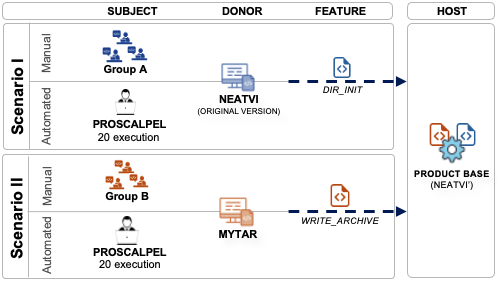
\includegraphics[width=9cm]{images/experiment_design7.png}
	\centering 
	\caption{Experiment design: one factor with two treatment applied in two re-engineering scenarios.}
	\label{fig:experiment_design}
\end{figure} 

%%%%The same process was automatically performed, following \FOUNDRY approach supported by \autoscalpel. To achieve the time and accuracy of \autoscalpel, we computed the average runtime of 20 runs transplanting a new feature variant to the product base for each scenario. Then, we report the number of \autoscalpel runs in which all test cases passed in the successful running.  


%For each run, we evaluate the degree to which the transplantation was successful by applying the same test cases and test suites used to evaluate the resulting product line generated by the participants.
 
%%%The other instrument is the system size; small features are used in this experiment in place of the features presented in last study. We assume that inspecting the code to transfer a feature to a product line is hard, slow, and possibly a tedious work. Thus, we preferred this way to avoid participant's tired, in another way, it would require too much time of execution. Further details on the operationalisation and instrumentation of this construct is presented later in the paper.
%%As we know, preparing a experiment with a manual processo of product line generating considering large code bases would be too difficult and slow process for an in-lab study. Thus, we opted by use small systems as donor systems, since it has been a scenario when our automated approach could not prove its real gains.

%%%As we know, comparing our automated approach with a manual ones as baseline considering large code bases would be too difficult and slow for an in-lab study. Thus, we opted by use small systems as donor systems, since it has been a scenario when our automated approach could not prove its real gains.

%%%As we know, preparing a experiment with a manual process of product line generating considering large code bases would be too difficult and slow process for an in-lab study. Thus, we opted by use small systems as donor systems, since it has been a scenario when our automated approach could not prove its real gains.
%%We identified the \emph{write\_archive} feature from MYTAR and \emph{dir\_init} feature from NEATVI for transplantation. 

%%Aiming to assess \FOUNDRY with respect to human effort, we conducted an experiment based on Wohlin et al.~\cite{Wohlin2012}, that reflects a real-world process of feature reuse. 
%%The design \emph{one factor with two treatments}~\cite{Wohlin2012} was used in each scenario, in which we compare the two treatments in relation to each other. The factor is the type of the approach used. For the first treatment, we tested the manual approach performed by the subjects. For the second, we tested the approach proposed in this work. For both treatments, the data used in the tests were the same, so as to avoid possible bias. 

%%%We computed the accuracy of our approaches and the time needed for transferring features to the product base in comparison with the subjects results.
%%The experiment design is showed in Figure~\ref{fig:experiment_design}.

The way used to perform the feature transferring process during the experiment represents an independent variable with two levels, manual and automated. We also distinguish participants related to the instrumentation they use: a group A, executing on scenario I and a group B, executing the scenario II. 

In this experiment, the dependent variables are the accuracy product line generation process and the payoff for using or not our approach. That is, to analyze the accuracy of the approach (RQ1), we evaluate the degree to which a transplant was successful for generating a product line. To analyze the performance of the approach (RQ2), we measured the time spent by participants to extract, adapt and merge one feature from each donor system. 

%%For each scenario, we repeat each run 20 times. Then, we report the number of \autoscalpel runs in which all test cases passed in the successful running.  

%%%%Thus, our test cases check whether or not the output of the feature is correct with respect to the original donor systems, rather than just checking the exit code.




%We proposed the extraction of one feature from each system by each group. The feature transplanted in the first scenario (group) must be small than the second one, given the limitation of the participant's time and effort required to adapt the feature to be reused in a distinct codebase. The pilot served to align them.
%We also distinguish participants related to the donor systems they use: MYTAR and NEATVI systems.



%We measured the average time spent on feature transplantation using \autoscalpel 20 times. 
%We also computed the manual effort of the participants to transfer these some feature in a product base. 


%%While participants are running the experiment, we ask them to verbalize their thoughts informing us which support strategies were being used for each stage of the features transfer process. (Protocol to think aloud [11]). When necessary, we also ask why they are performing a specific activity. The think-aloud protocol allowed us to capture data strategies and performance data simultaneously, instead of waiting until the experiments finishes to take these data. In addition, we provide an activity and time registration worksheet. We run the experiment for one participant at a time.

\subsection{Pilot Study}

Before the simulation process, we conducted two pilot studies with 6 graduate students. We used the pilot study results to determine the amount of time needed to execute our tasks and the suitable size of features. This allowed us to estimate and plan the number of participants we needed in the main study. 

The pilot study also allowed us to assess whether the participants could properly understand the subject systems and the tasks they should perform. We do not consider the results of the pilot in our analysis.

\subsection{Participants}

After the pilot, we recruited 20 participants (excluding pi-lots): 2 undergrads (Un), 9 masters (M), 7 PhD. (PhD), and 2Post-Ph.D. (Post-PhD). Most of them have more than 5 years of SPL experience and 10 years of software development. The participants are from ten different universities (from U1to U10) and the analysts/developers work in four different companies (C1, C2, C3, C4 and C5). To recruit them, we sent emails to professors in two universities, from different software reuse research groups, to suggest current and ex-members. 

Before the experiment, we asked them to answer an online survey, which we used to collect background data about their experience, mainly in software development and SPL. According to our design, we created balanced groups(A and B) of participants to each product line generation scenario based on their experience. Table~\ref{tab:participants} shows the details of the participants involved in the experiment.

\begin{table}[t]
\centering 
	\caption{\textit{Details of participants' expertise (in years) and division into groups. Group A worked on scenario I, transplanting a feature from different versions of the same donor system as the host. Group B worked on scenario II,transplanting a feature from a donor system different to the host one}}
	\label{tab:participants}
	\resizebox{7cm}{!}{%
	\begin{tabular}{clllll} \hline
%	\toprule
		Group &Part. &Degree & Inst. & \multicolumn{2}{c}{Exp. (years)}\\ \cline{5-6}
		              &         &  &   & Dev.      &  SPL     \\\hline
		A       &P1  & MSc     & U7   & [1,5)     &  [5,10)  \\%magno
    	        &P2  & Un      & C5   & [10)      &  [1,5)   \\%mateus
		        &P3  & PhD     & U4   & [10)      &  [10)    \\%jonatas
		        &P4  & MSc     & U4   & [10)      &  [1,5)   \\%marco
		        &P5  & MSc     & U4   & [10)      &  [5,10)  \\%Djan
		        &P6  & MSc     & U4   & [10)      &  [5,10)  \\%Renata
		        &P7  & PhD     & U8   & [10)      &  [10)    \\%Alcemir
		        &P8  & PhD     & U9   & [10)      &  [1,5)   \\%Tiago
	            &P9  & Pos-PhD & U10  & [10)      &  [10)    \\%Larissa
	            &P10  & PhD     & U4   & [1,5)     &  [1,5)   \\\hline%Stefani
	            
		B       &P11   & MSc     & C1   & [10)      &  [1,5)   \\%Daniel
	            &P12   & MSc     & C2   & [1,5)     &  [1,5)   \\%Rose
		        &P13   & Un      & C3   & [10)      &  [1,5)   \\%Taijara
		        &P14   & PhD     & U1   & [10)      &  [10)    \\%Michele
		        &P15   & PhD     & U2   & [10)      &  [10)    \\%Paulo
		        &P16   & PhD     & U3   & [10)      &  [5,10)  \\%Tassio 
		        &P17   & MSc     & U4   & [5,10)    &  [5,10)  \\%Rafael X
		        &P18   & MSc     & C4   & [5,10)    &  [5,10)  \\%Anna
		        &P19   & PhD     & U5   & [10)      &  [10)    \\%Iuri
		        &P20  & MSc     & U6   & [5,10)    &  [1,5)   \\\hline%Loreno 
		        
	\end{tabular}
	}
\end{table}

\subsection{Operation}

Before the participants receive their tasks, we introduced the experiment with a \emph{tutorial} about clone-and-own and reengineering of existing systems into SPL. The tutorial took 30 minutes on average.

%In general, we asked the participants to use their knowledge in C and SPL to identify, extract, adapt and deploy each feature into the same product base. 
We provided the participants with the same input as the one required for \FOUNDRY, namely: feature entry points in the donor, a set of automated unit testing, the donor’s source code, and a prepared product base with the target insertion point. Additionally, they received a few-sentence description of each feature in the target system and the system’s documentation with donor and host feature models. From those artifacts, they get domain knowledge about the systems. 
%From those artifacts, they get knowledge about the systems and how to perform the reengineering process.

The direct costs of this experiment are related solely to the time spent by the researcher with setup of the experiment itself. This involved: specifying the respective annotations for the entry point and insertion points of the features, which took approximately 13 minutes of work at the scenario I and 17 minutes at scenario II; creating the test cases, necessary to validate the target features, taking approximately 16 minutes of programming activities; preparing the product base, which took approximately 14 minutes; then, approximately 34 minutes were spent creating all documentation of donor systems including the product base feature model.

To extend the number of product base variants with a new feature transferred from the correspondent donor system, all participants had three activities based on clone\&own and the migration of cloned variants to a product line~\cite{Krueger2001,Mahmood2021}: feature \emph{extraction}, \emph{adaptation} and \emph{merging}, with descriptions and instructions provided for each task.  

Initially, the participants must identify and extract all code associated with the feature of interest to a temporary directory. Each portion of code identified as belonging to the target feature must be involved with $\texttt{\#ifdef}$ directives. For example, $\texttt{F\_DIR\_INIT}$ for the feature $\texttt{dir\_init}$. Then, the participant must rewrite extracted feature to it executes correctly in the product base environment, passing in all unit tests. To  be  more  precise, the participant has to change the feature source code to be compatible with the name space and context of its target insertion point in the product base. Finally, the participant must insert the feature code into the product base environment to validate the correctness of the feature at the emergent product line. 
%The target site in the product base was provided by us

%%If compared with approaches relying on pure machine learning algorithms, our approach needs some extra effort in order to be executed, such as: definition of the assignment rules and extraction of context information. In the context of SERPRO, although the retrieval of context information was straightforward, some extra work was necessary to insert this information in the database used by our approach. Thus, with this information in hands, we computed that 2 hours was necessary for processing and integrating the context information in the approach. In regarding to the definition of the rules, we spent about 36 hours. This involved the manual analysis and statistics of CR data, just as described in the operation. Thus, we spent a total of 38 hours for the preparation of our approach prior to the experiment’s execution.

%With respect to time needed to train the SVM algorithm, it was the same for both approaches. This was actually expected because both approaches use the same algorithm and the treatments were ran with the same dataset. Therefore, we did not consider this in our analysis since it would not change the results.

%%For each code element identified the participants must to envolve it with \#ifdef directives. Together, these scenario inset a new variants to our product base.


\subsection{Data collecting}

We have provided a task and time registration worksheet. While participants were running the experiment, we ask them to take notes of which strategies were being used for each stage of the features transfer process and why they are performing each specific task. It allowed us to capture strategies and performance data simultaneously. 

We have complemented the above setup with a post-survey. By post-survey, we could better understand participants' difficulties and meaningful differences about the manual and automated process in both scenarios. We have triangulated the data generated with the experiment with the responses we obtain from the pre and post-survey.

To establish the time for feature transplantation using our automated approach concerning manual effort, we ran \autoscalpel 20 times, and measure the average time transplanting the same feature used by the participants in each scenario. This average time was compared with the time spent by our participants on the manual re-engineering process. 

Based on our pilot study, we set a time limit of 4 hours for each manual and automated process. Another way, the result might be affected negatively by participants' boredom and tiredness. 
%The other instrument is the system size; small features are used in this experiment in place of the features presented in last study. We assume that inspecting the code to transfer a feature to a product line is hard, slow, and possibly a tedious work. Thus, we preferred this way to avoid participant's tired, in another way, it would require too much time of execution. Further details on the operationalisation and instrumentation of this construct is presented later in the paper.

%%%\subsection{Data analysis}

%%Our quantitative analysis strategy aims to build a reliable set of evidence based on the application of statistical methods. The results for each dependent variable constitute a sample, therefore, the first analysis step consists of identifying the statistical distribution for each sample through the Shapiro-Wilk~\cite{Shapiro1965} method. Its null hypothesis claims the population as normally distributed.

%%For the analysis we compared the average time of our 20 execution of \autoscalpel and the average time of the participants in the experiment. For the statistic analysis of our data, we conducted an analysis of variance using a between-subjects ANOVA. It is a parametric test for determining whether significant differences occur in an experiment containing two or more conditions. 


%CONTINUE....
%%For the qualitative analysis, we analysed the sheets and listened to the audios (post-interview) looking for commonalities and differences in the way participants execute the tasks and their perception about the manual process. We transcribed participants answers and informally generated codes to passages of the data which are relevant to understand participants difficulties and meaningful differences about the approaches used.

%%Source code. Different coding conventions used in software systems may lead to wrong conclusions. For this reason, we preprocessed the analyzed software systems by eliminating comments, empty lines, and include guards, and by applying source code pretty printing

\subsection{Results and Discussion}

We used 22 pre-existing regression test suite designed by the \emph{NEATVI} developers to assess the accuracy of \autoscalpel and answer our \textbf{RQ1}. However, they were not designed to test  \emph{NEATVI} as a product base with new variants and may not be sufficiently rigorous to find regression faults introduced by the re-engineering process. To achieve a better product line coverage, we manually augmented the host’s regression test suites with additional tests, our augmented regression suites. 

Furthermore, we implemented an acceptance test suite with 3 tests cases for evaluating the transferred feature in the scenario I and 2 for evaluating the feature in scenario II. Thus, we executed a total of 27 tests in the scenario I and 29 in scenario II, considering the acceptance tests already incorporate into the product base by the first variant inserted in scenario I. 

We summarise our results in Table~\ref{tab:transplantation_results}.  We report the status of the product base and variant inserted by the participants, the time spent and the number of passing tests for the regression augmented regression and acceptance test suites. In the first scenario, only one of the participants was not able to finish the process before the timeout. On the other hand, half of the participants were able to finish the process before achieving the timeout in the second scenario and only three of them have been able to insert the target feature without breaking the product base. 

\begin{table*}[t]
\centering 
    \caption{Experiment results comparing the time of tool over 20 repetitions with the participants:column product line status shows the generated product line status by participants and tool; column \emph{Execution Time} shows the time spent on the feature transplant by the participants and the average time of 20 run of \autoscalpel, we highlight the execution time of the participant that spent less time; column \emph{Test Suites} shows the results for each test suite; columns \emph{PASSED} report the number of passing tests; \emph{ALL} report the percent of test passed for the postoperative product line; and \emph{COV.} report statement coverage (\%) for the postoperative host and for the organ.}
	\label{tab:transplantation_results}\small
	\resizebox{18cm}{!}{%
	\begin{tabular}{llrrrrrrrrrrrrr}\\\hline
		\multicolumn{1}{c}{}      &&&    & \multicolumn{9}{c}{Test Suites}                                                                  \\
		\cline{5-9} \cline{10-13} 
		\multicolumn{1}{c}{Scenarios} & \multicolumn{1}{c}{Participants} & \multicolumn{1}{c}{ Product Line} & \multicolumn{1}{c}{Execution}& \multicolumn{3}{c}{Regression} & \multicolumn{3}{c}{Regression++.} & \multicolumn{3}{c}{Acceptance} \\
		\multicolumn{2}{c}{} & \multicolumn{1}{c}{Status} & \multicolumn{1}{c}{Time (minutes)} & \multicolumn{1}{c}{PASSED} & \multicolumn{1}{c}{ALL\%} & \multicolumn{1}{c}{COV.\%} & \multicolumn{1}{c}{PASSED} & \multicolumn{1}{c}{ALL\%} & \multicolumn{1}{c}{COV.\%} & \multicolumn{1}{c}{PASSED} & \multicolumn{1}{c}{ALL\%} & \multicolumn{1}{c}{COV.\%} \\\hline

		 \multirow{10}{*}{II} & P1 &\multicolumn{1}{l}{OK}      &\textbf{82}  & 22 &100 &-- &2 &100 &-- &3 &100 &--\\
		    & P2 &\multicolumn{1}{l}{OK}      &\textbf{88}  & 22 &100 &-- &2 &100 &-- &3 &100 &--\\
		    & P3 &\multicolumn{1}{l}{OK}      &\textbf{77}  & 22 &100 &-- &2 &100 &-- &3 &100 &--\\
		    & P4 &\multicolumn{1}{l}{OK}      &\cellcolor[gray]{.9}\textbf{68}  & 22 &100 &-- &2 &100 &-- &3 &100 &--\\
		    & P5 &\multicolumn{1}{l}{OK}      &\textbf{81}  & 22 &100 &-- &2 &-- &-- &3 &100 &--\\
		    & P6 &\multicolumn{1}{l}{Broken} & \multicolumn{1}{l}{\textbf{Timeout}}   & 0 &0  &--   &0 &0 &--   &3 &0 &--  \\
		    & P7 &\multicolumn{1}{l}{OK}      &\textbf{87}  & 22 &100 &-- &2 &100 &-- &3 &100 &--\\
		    & P8 &\multicolumn{1}{l}{OK}      &\textbf{83}  & 22 &100 &-- &2 &100 &-- &3 &100 &--\\
		    & P9 &\multicolumn{1}{l}{OK}      &\textbf{73}  & 22 &100 &-- &2 &100 &-- &3 &100 &--\\
		    & P10 &\multicolumn{1}{l}{OK}      &\textbf{113} & 22 &100 &-- &2 &100 &-- &3 &100 &--\\
		 \hline 
		 
		 \rowcolor[gray]{.9} & \textbf{\autoscalpel} &\textbf{OK in 20/20 runs} &\textbf{20} &\textbf{22} &\textbf{100} &\textbf{--} &\textbf{2} &\textbf{100} &\textbf{--} &\textbf{3} &\textbf{100} &\textbf{--}\\
		 \hline
		\multirow{10}{*}{I} & P11 &\multicolumn{1}{l}{Broken} & \multicolumn{1}{l}{\textbf{Timeout}}  & 0 &0  &--   &2 &0 &--   &0 &0 &--   \\
		 & P12 &\multicolumn{1}{l}{Broken}  & \multicolumn{1}{l}{\textbf{Timeout}} & 0 &0  &--  &2 &0 &--   &0 &0 &--   \\
		 & P13 &\multicolumn{1}{l}{Error}    &\textbf{181} & 0 &0  &--   &2 &0 &--   &0 &0 &--   \\
		 & P14  &\multicolumn{1}{l}{Broken} &\multicolumn{1}{l}{\textbf{Timeout}}   & 0 &0  &--   &2 &0 &--   &0 &0 &--   \\
		 & P15 &\multicolumn{1}{l}{Broken}  &\multicolumn{1}{l}{\textbf{Timeout}}   & 0 &0  &--   &2 &0 &--   &0 &0 &--   \\
		 & P16 &\multicolumn{1}{l}{Error}    &\textbf{114} & 0 &0  &--   &2 &0 &--   &0 &0 &--   \\
		 & P17 &\multicolumn{1}{l}{OK}       &\cellcolor[gray]{.9}\textbf{104} &25  &100 &-- &2 &100 &-- &2 &100 &-- \\
		 & P18 &\multicolumn{1}{l}{OK}       &\textbf{194} &25  &100 &-- &2 &100 &-- &2 &100 &-- \\
		 & P19 &\multicolumn{1}{l}{OK}       &\textbf{131} &25  &100 &-- &2 &100 &-- &2 &100 &-- \\
		 & P20 &\multicolumn{1}{l}{Broken} & \multicolumn{1}{l}{\textbf{Timeout}} &0   &0  &--   &2 &0 &--   &0 &0 &--   \\
		 \hline 
		 \rowcolor[gray]{.9} &\textbf{\autoscalpel} &\textbf{OK in 19/20 runs} &\textbf{27} & \textbf{25} & \textbf{100} & \textbf{--} &\textbf{2} &\textbf{2} &\textbf{--}  &\textbf{2} &\textbf{100} &\textbf{--}\\\hline

	\end{tabular}
}
\end{table*}

For each scenario, we also report the number of \autoscalpel runs in which the product derived passed in all test cases in the successful running. For each scenario, we repeat each run 20 times. The success rate was retained for both scenarios I and II, where we lost only one successful run in the timeout and the product line generated passed in all tests in all test suites.

\begin{framed}
\noindent To answer \textbf{RQ1},the results show success of  rate was retained for both scenario I and II, where we lost only one successful run in the timeout and all products derived passed in all test in all test suites.  
\end{framed}

As stated in the definition of the metric \textbf{M2} and to answer \textbf{RQ2}, we evaluate the payoff of \FOUNDRY. Figure~\ref{fig:experiment_result_time_II} graphically shows the time spent on each activity performed in re-engineering to SPL process. In summary, Group A transferred the target feature from \emph{NETVI} to the product base in 1h24 minutes on average. \autoscalpel turned out to be quicker, successfully transplanting this feature in all 20 trials, in an average of 20 minutes.

\begin{figure}[t]
	\centering 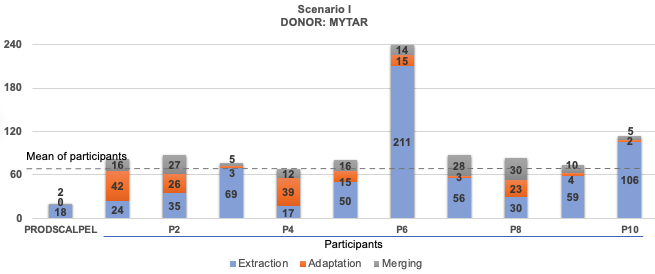
\includegraphics[width=8.5cm]{images/experiment_result-SC1-4.png}
	\label{fig:experiment_result_time_I}
\end{figure} 
\begin{figure}[t]
	\centering 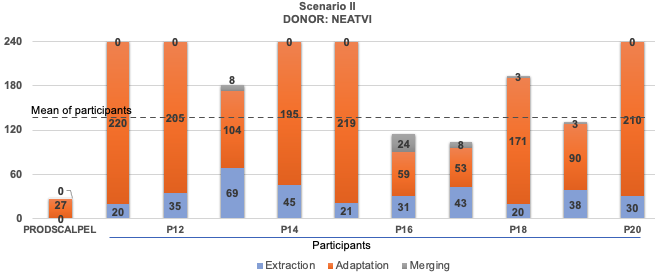
\includegraphics[width=8.5cm]{images/experiment_result-SC2-4.png}
	\centering \caption{Time (in minutes) spent by participants and \autoscalpel on performing the three stages of SPL reengineering: feature \emph{extraction}, \emph{adaption} and \emph{merging}. The graph highlight the average participants time that successful generated its target product line.} 
	\label{fig:experiment_result_time_II}
\end{figure} 

Most of the participants of Group B had not completed the product line generation process from \emph{Mytar}  within the 4 hours time limit. Considering the participants that were able to finish the process (i.e., participants \emph{P17}, \emph{P18} and \emph{P19}) and its product line passed in all test suites they spent an average of 2h23 minutes while \autoscalpel was able to complete this task in 19 of 20 trials in the timeout, taking 27 minutes on average.

\textbf{Statistic analysis of performance.} The quantitative analysis strategy from the experiment was adapted to this study because there is no comparison between scenarios since used different donors and target features. The first analysis step consists of identifying the statistical distribution for each scenario through the Shapiro-Wilk~\cite{SHAPIRO1965}, a method with the best power for a given significance~\cite{Razali2011}. Its null hypothesis claims the population is normally distributed. It determines which set of methods must be applied in the hypothesis testing and the strength of association between variables. 

Figure~\ref{fig:experiment_result_boxplot} graphically shows the time results for our two groups in comparison with \autoscalpel performance. In the scenario, I, the preliminary information provided by the box plots indicate that all samples are normally distributed (W = 0.70445, p-value = 3.129e-05). Thus, a ANOVA~\cite{Gelman2005} and Pairwise Student’s t-test analysis were conducted considering the hypothesis of the time values for \autoscalpel have statistically higher values if compared to the manual methods (p-value $<$ 2e-16). It led to the rejection of the null hypothesis for all pairs. 

In the scenario II, the normality test result showed a normal distribution with a W = 0.69378, p-value = 1.715e-06. Thus, we used ANOVA to hypothesis testing and Pairwise t-Student. Based on the ANOVA test and Pairwise t-Student, we rejected the null hypothesis (p-value $<$ 2e-16) that the distribution of the population is homogeneous.

We can concludes that \autoscalpel reduces developer effort to transfer features to a product line in both scenarios. For both simulation scenarios, there is a significant effect size between the tasks performed in a manual way and using \autoscalpel. The participants had similar performance times in scenario I, with the exception of the participants \emph{P6}. On the other hand, most of the participants of scenario I do not terminate the experiment before the 4-hour timeout. This last one is qualitatively explained by the participants in the post-survey where they exposed how 
hard is to adapt a feature to run in a strange codebase. 
 
\begin{figure}[t]
	\centering 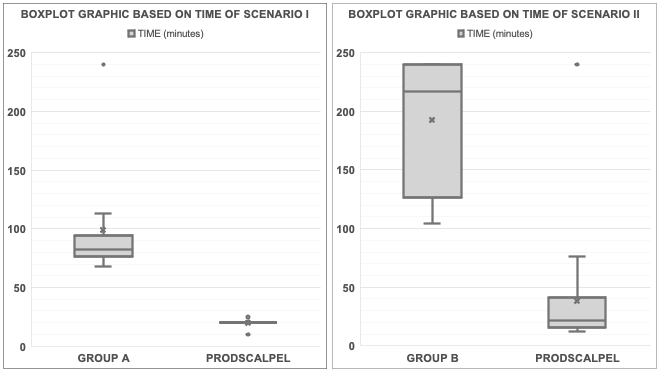
\includegraphics[width=8.9cm]{images/experiment_time_results.png}
	\centering 
	\caption{Time results grouping automated and manual in both scenarios.  Scenario I: \emph{NEATVI} - Product Base; Scenario II: \emph{Mytar} - Product base.}
	\label{fig:experiment_result_boxplot}
\end{figure} 


\begin{framed}
\noindent To answer \textbf{RQ2}, in both scenarios \autoscalpel outperformed participants with respect to the average task time. By considering the sum of time spent with both scenarios, the tool accomplished the product line generation process  by inserting two new variants in 4.8 times faster than the mean of participants were able to finish the experiment in the timeout and their resulting product line passed in all test cases.
\end{framed}

\section{Threats to Validity}

The threats to the validity of this study are mainly related to external and internal validity~\cite{Wohlin2012}. Conclusion validity issues involve the low power of the statistical analysis. The number of SPL projects can be a threat to the hypotheses not rejected in this experiment. Aiming to address it, the extension of the experiment to incorporate new donors systems is being explored, and improved results will be reported in future work. In addition, we already provide a set of heterogeneous systems, with distinct characteristics in terms of domains, amount of code lines, and numbers of features. It provides a representation on how the \autoscalpel approach behave when applied to different objects as an archive manager providing features to generate a text editors product line.

\textbf{External Validity.} The relatively small number and diversity of systems used for generating a product line pose an external threat to validity. We applied our results to small programs due to the boundaries of an in-lab study; our results may not generalize to larger programs in the wild. We tried to mitigate it by constructing possible real-world scenarios, i.e., reuse of features from unrelated codebase and variations of the same systems, both real-world systems. Additionally, given that our approach was helpful even in small programs, we argue that is likely helpful for larger systems as it is nearly impossible to incorporate new variants to a product line without a large understanding of the donor systems specifications or without specialized tool support~\cite{Assuncao2017}.

%Justyna: I don't want to draw attention to that.
%\textbf{Construct Validity.} We did not compare our tool using a real-world SPL extracted from NON-SPL as a baseline. A critical part of the validation of a tool for SPL reengineering from existing systems is to find a suitable baseline that defines a transition process between NON-SPL systems codebases to an  SPL or even a tool that performs such process with codebases written in C. Although the task without specialized tool support is too difficult and slow, it is useful as a baseline to investigate the benefits of \FOUNDRY by provide an automated solution to the process. 

\textbf{Internal Validity.} Due to time expensive nature of a human study, we had few participants. We tried to mitigate this issue by selecting participants with considerable experience in SPL projects. The other threat to the validity is the system size; small features are used in this experiment. We assume that inspecting the code to transfer a feature to a product line is hard, slow, and possibly a tedious work.  Thus, we preferred this way to avoid eventual human error as consequence of participant's tired, in another way, it would require too much time of execution. Even with a limited execution time, we were able to transplant features from donors with significant size (consisting the more than 6k LoC of our donor systems together, as shown in Table~\ref{tab:instrumentation}. We also use testing as means of validating our approach, which cannot provide a formal proof of its correctness.  We used extensive testing to mitigate this risk. Moreover, testing is a standard approach to code evaluation in real-world scenarios due to its high scalability.
\section{Related Work} \label{sec:related_work}

There are four research areas relevant to this work, namely reengineering of systems into SPL, clone-and-own, search-based software engineering, and software transplantation.

%\subsection{Reengineering for \ac{SPL}}
\textbf{Reengineering of Systems into SPL}. Diverse academic proposals and industrial experience reports addressing reengineering for extractive SPL are present in the literature, as shown in Assuncao et al.’s mapping study~\cite{Assuncao2017}. However, this number decreases considerably when we are interested in proposals that automate the lifecycle of the reengineering process~\cite{Kruger2020}. In many papers, the authors expose only an intention to provide a tool support for their approaches. Some initiatives have been providing solutions for reengineering product family into a configurable product line~\cite{Faust2003, Mende2008, Koschke2007}. Others provide support for specific tasks~\cite{Martinez2015, Alves2007, Nunes2012, Klatt2014, Tang2015}. These studies can provide interesting solutions to reengineering practices. Nevertheless, unlike FOUNDRY, such approaches do not adapt target features automatically. Moreover, the feature integration in an SPL is semi-automatic, while FOUNDRY requires no effort from the developers for this process.

Ziadi et al.~\cite{Ziadi2014} introduces \emph{But4Reuse}, an extraction-based technique for product-line migration, including support for feature-model synthesis. But4Reuse has the advantage of working on various cases (different programming languages and artifacts) thanks to its adapters system. However,  variability within the body of methods or functions (i.e. the statement level), which causes significant duplicates in the different features of their SPL representation. Finally, the maintenance and evolution can only be done by re-extracting the entire product line after modifying the products. With \autoscalpel, we allow developers to directly manipulate an SPL implementation through their over-organs, which are accessible for them possible to be individually maintained and tested, for example, using unit testing approaches with the original feature playing the role of oracle.

\emph{IsiSPL}~\cite{hlad2021} is a reactive approach to SPL adoption in the software industry. IsiSPL automates the integration and generation phases in a non-invasive development cycle. However, it proposes a representation of an SPL implementation in the form of an annotated code, what have impact on the code comprehension, even performing a simplification that removes redundant annotations.

%\subsection{Clone-and-own}
\textbf{Clone-and-own}. Clone-and-own was proposed as a simple alternative to SPL~\cite{Dubinsky2013, Fischer2015, Krinke2010, Ray2012, Martinez2015, Stanciulescu2015}. 
It is an ad hoc reuse practice that creates new products in a software family by copying and adapting an existing product~\cite{Dubinsky2013, Fischer2015}. \FOUNDRY also can be exploited as an automated alternative to clone-and-own approach to the optimization of the product development process, where it is used as a one-off to create a new product. Although there are tools for feature location from code-and-clone detection techniques, the adaptation of feature to reuse still requires manual work~\cite{Yoshimura2006, Kastner2014}. 

Fischer et al.~\cite{Fischer2015}, for instance, present \emph{ECCO} to enhance clone-and-own. The tool finds the proper software artifacts to reuse and then provides guidance during the manual completion by hinting at which software artifacts may need adaptation. Like \autoscalpel, ECCO also produces a black-box representation of a product line implementation, with no annotated code, which easily the maintenance process of its product line. However, ECCO requires that its features source must be based on the same family of products which limits the capacity of reusing assets. Furthermore, ECCO considers the code in the body of methods as raw lines, each line of code being a new artefact, which complicates the evolution process of an SPL. Whereas in FOUNDRY, the product line representation stores an over-organ that can be automatically "pruned" to be adapted to different products variation. Additionally, \autoscalpel relies on a clone detector to deal with the variability relationship, namely the implication, the mutual exclusion, the co-occurrence, and the common and optional feature. This means that \autoscalpel recognize these relationships independently of the human intervention or by requiring any other artefact besides the source code.

\textbf{Search-based Software Engineering}. In their keynote paper, Harman and colleagues advocate the potential the application of search-based algorithms, as genetic improvement~\cite{Petke18:genetic}, for SPL development~\cite{Harman2014a}, for instance, in migrating products into an SPL~\cite{Rubin2013b, Fischer2014}. Harman et al. present a survey with directions for future work on SBSE with applications in SPL~\cite{Harman2014a}. Regarding the re-engineering process, the authors present some research on reverse engineering of feature models, applying search-based techniques. Since then, new studies~\cite{Segura2013,  Linsbauer2014, Lopez2015}  applying search-based algorithms for feature model generation appeared. We are the first to propose an approach and evaluate a tool for SPL migration using SBSE.

\textbf{Software Transplantation}. As far as the literature on automated software transplantation is concerned, Petke et al.~\cite{Petke2014,Petke2018} were the first to transplant snipets of code from various versions of the same system to improve its performance, using genetic improvement~\cite{Petke18:genetic}. One year later, Barr et al. successfully transplanted a feature from one program into another~\cite{Barr2015}. 
More recently, Petke et al.~\cite{Petke2018} used transplantation for genetic improvement-based specialisation. In contrast, we explore multi-organ ST for SPL generation. We focus on how transplantation can be used for extracting the intended code from different donors, inserting a variability mechanism and deploying it in a prepared product base in order to build product lines or new products.


\section{Conclusions and Future Work} \label{sec:conclusion_future_work} 

In this work, we propose an approach, \FOUNDRY, and a tool, \autoscalpel, for product line migration by reusing existing codebases with minimal human involvement. Both approach and the tool have been validated through case studies\footnote{We will provide a replication package in case of acceptance}. We generated two product lines and two products through the transplantation of features extracted from three real-world systems into two different product bases. Additionally, we performed an experiment with SPL experts to compare our approach with manual effort, showing significant time effort improvements when using \autoscalpel. The tool accomplished the product line generation process by inserting two new variants 4.8 times faster than the mean of participants who were able to finish the experiment in the timeout.

We argued that the migration into a transplantation-based—in contrast to an annotation-based—software product line makes it usable in practice, improves maintainability due to physically separated features, and guarantees to preserve semantics.  \FOUNDRY approach can be used both to \emph{extractive} or \emph{reactive} product line migration strategy, as a systematic Clone\&own strategy to specialize existing products, avoiding the duplication of feature implementations, preserving features behavior, reduce feature redundancy, and automating changes propagation. That is, solutions for problems often cited in both SPL and clone\&own literature.

Our evaluation studies provide initial evidence to support the claim that automated product line generation, using the transplantation idea, is a feasible and, indeed, promising direction for software development with minimal human involvement. However, more studies are needed to provide more evidence for generalisability of the approach in a different domain, and that also considers its application in an industry context.


\appendices
\section{Proof of the First Zonklar Equation}
Appendix one text goes here.

\section{}
Appendix two text goes here.

% use section* for acknowledgment
\ifCLASSOPTIONcompsoc
  % The Computer Society usually uses the plural form
  \section*{Acknowledgments}
\else
  % regular IEEE prefers the singular form
  \section*{Acknowledgment}
\fi


The authors would like to thank...

\ifCLASSOPTIONcaptionsoff
  \newpage
\fi

\bibliographystyle{IEEEtran}
\bibliography{biblio}

\begin{IEEEbiography}{Author name}
Biography text here.
\end{IEEEbiography}

% if you will not have a photo at all:
\begin{IEEEbiographynophoto}{Author name}
Biography text here.
\end{IEEEbiographynophoto}

\begin{IEEEbiographynophoto}{Author name}
Biography text here.
\end{IEEEbiographynophoto}

% that's all folks
\end{document}


